\chapter{深度学习的正则化}
\label{chap:7}
%%%%%%%%%%%%%%%%%%%%%%%%%%%%%%%%%%%%%%%%%%%%%%%%%%%%%%%%%
%%%%%%%%%%%%%%%%%% author:ysh329 %%%%%%%%%%%%%%%%%%%%%%%%
%%%%%%%%%%%%%%%%%%%%%%%%%%%%%%%%%%%%%%%%%%%%%%%%%%%%%%%%%
机器学习的一个核心问题是如何使算法在除训练集以外的新输入数据上的性能表现更好。机器学习的不少学习策略都被用来去减少测试误差,有的策略会以牺牲训练误差为代价减少测试误差。这些学习策略都统称为正则化方法。对于深度学习从业者来说,有很多正则化的方法可以使用。实际上在深度学习领域,设计并开发更有效的正则化方法已成为一个主要的研究方向。

本书第五章介绍了泛化,欠拟合,过拟合,偏差,方差以及正则化的基本概念。在继续本章的内容之前,如果您还对这些概念不了解,可以参考第五章的具体内容。

本章节将会详细地介绍正则化方法,关注正则化方法在深度模型以及为深度模型搭建提供子模块模型上的应用。

本章的部分小节将会提到机器学习中的标准概念。如果您熟悉这些概念,可以跳过与之相关的小节。但是本章的大部分内容都是这些基本概念的延伸或扩展,尤其是有关神经网络的相关案例。

在5.2.2小节给出正则化的定义:“用于修正学习算法减少泛化误差而不是训练误差的策略”。

其中讲到一些正则化方法,某些正则化是基于机器学习模型加入额外限制实现,例如给参数加上限制。某些方法则是在目标函数中加入多余的项,多余的项可以视为对应参数的软性限制。如果正则化方法选择合理,额外的限制和惩罚可以提升模型在测试集上的性能表现。一方面,这些额外的限制和惩罚是作为编码先验知识的一种形式;另一方面来说,这些额外的限制和惩罚被设计出来用于提升模型的泛化能力。有时因为惩罚和限制的存在,可以使原本不确定的问题变得确定。此外,还有其它形式的正则化方法,例如众所周知的集成方法,基于训练数据将多个假设合成一个模型。

在深度学习的背景下,大多数正则化策略都是基于正则化估计。正则化估计通过平衡偏差和方差来实现其作用,如减少方差增大偏差。一个有效的正则可以在显著减少方差的同时不会过分增大偏差。在第五章中讨论泛化和过拟合时,我们主要关注模型族训练过程中的三个情形:(1)排除真实数据产生过程中对应的欠拟合以及偏差增大,(2)真实数据的产生过程,(3)数据生成过程中也可能伴随其它数据的生成过程——导致模型步入过拟合阶段,其中相比偏差,方差是造成了估计误差的主要原因。正则化的目标好比是让模型从第三阶段到第二阶段。

在实际过程中,一个过度复杂的模型族并不需要包括目标函数或者真实数据的产生过程,或与之近似的过程。我们基本上从来都不知道真正数据的产生过程是怎么的,所以我们也就无法确定模型族里是否包含数据的真实生成过程。但是深度学习算法特别地被应用在复杂的领域,如图像、语音序列、文本,因为这些数据的真实产生过程好比模拟整个宇宙。从某种程度上来说,我们总在试图用一些有棱角的零件(即真实数据的产生过程)塞到圆孔(即模型族)中。

控制模型的复杂度不仅意味着发现模型真正的规模大小,还包括参数的规模大小。此外,我们有时也会发现在实际深度学习的应用场景中,(在最小化泛化误差的意义上)拟合最好的模型的特点,不仅是一个大模型,而且也使用了适当的正则化方法。

现在让我们回顾一下如何创建大规模、深层且使用了正则化的模型。

\section{参数范数惩罚}
在深度学习出现之前,正则化已被使用了十几年。线性模型中的线性回归模型、逻辑斯特回归模型都可以使用简单、直接且有效的正则化方法。

许多正则化方法都是基于有限的模型复杂度,如神经网络模型、线性回归模型、逻辑斯特模型,它们都是通过在目标函数$J$中增加一个参数范数惩罚项$\Omega (\theta)$,我们使用$\widetilde{J}$来表示加入正则化的目标函数:

$$
\begin{aligned}
	\widetilde{J} (\theta; X, y) = J(\theta; X, y) + \alpha \Omega (\theta)
\end{aligned}
$$

其中,$\alpha \in [0, \infty)$是一个超参数,用来平衡范数惩罚项$\Omega$的贡献度,也与标准的目标函数$J$有关。若将$\alpha$设置为$0$,那么不存在正则化项。更大的$\alpha$值对应更大的正则力度。

当训练算法正在对带正则化的目标函数$\widetilde{J}$求最小化时,基于训练数据集的原始目标函数$J$和参数$\theta$(或参数的子集)的大小的测量都将会减小。对于参数范数$\Omega$的不同选择将会导致不同的结果作为优选。在本节,我们将会讨论在模型参数上不同范数作为惩罚项的效果。

在深入研究不同范数作为正则的效果前,注意到对于神经网络通常会选择使用一个参数范数惩罚$\Omega$,它只会惩罚每层仿射变换的权重,偏置单元是不会被正则化的。偏置单元在拟合时所需要的数据量要小于权重。

每个权重明确表明两个变量之间是如何相互作用的。要将权重拟合地很好,需要在各种不同的条件下观察这些变量。每一个偏置只会控制一个单独的变量,这也就意味着在保留不被正则化的偏置时,不需要引入过多的方差。同样,对偏置参数进行正则化会引入相当程度的欠拟合可能。因此我们使用向量$w$来表明所有的权重,这些权重都会被范数惩罚所影响。其中,向量$\theta$表示所有的参数,既包括了所有的$w$以及没有被正则化的参数。

在神经网络的背景下,对于神经网络的每一层来说。因为在很多超参数的情况下搜索到正确的超参数值,代价很高。所以,在所有层中使用相同的权重衰减策略,用以减少搜索空间的规模,是情有可原的。

\subsection{$L^2$参数正则化}

在5.5.5小节中,我们已经看到了一种简单且最常见的参数范数惩罚法:$L^2$参数范数惩罚法,也是众所周知的权重衰减(weight decay)。该正则化策略通过在目标函数中加入一个正则化项$\Omega(\theta) = \frac{1}{2} ||w||_2^2$可以使权重越来越接近原本的值(一般来说,我们可以将参数正则化到空间中任何特定值的附近,令人惊讶的是,在收到正则化的作用后,可能会得到一个比之前更好的更接近真实值的结果。零是一个默认值是有意义的,当不知道正确值是正还是负时,零都会作为一个有意义的默认值。因为将模型参数正则化趋向于零是很常见的,我们也将重点关注这种特殊情况)。

在其它一些学术界,$L^2$被称为岭回归(ridge regression)或吉洪诺夫正则化(Tikhonov regularization)。

我们深入了解权重衰减的正则化方法,它的实现是通过学习正则化过的目标函数的梯度。为了简化说明,假设不存在偏置参数,所以$\theta$就相当于$w$,该模型有如下的目标函数:
$$
\begin{aligned}
	\widetilde{J} (w; X, y) = \frac{\alpha}{2} w^T w + J(w; X, y),
\end{aligned}
$$
其对应的参数梯度为:
$$
\begin{aligned}
	\triangledown_w \widetilde{J}(w;X,y) = \alpha w + \triangledown_w J(w;X,y)
\end{aligned}
$$
下面是单步梯度的权重更新:
$$
\begin{aligned}
	w \leftarrow w - \epsilon (\alpha w + \triangledown_w J(w; X, y)).
\end{aligned}
$$
也可以换个写法:
$$
\begin{aligned}
	w \leftarrow (1 - \epsilon \alpha)w - \epsilon \triangledown_w J(w; X, y).
\end{aligned}
$$
我们可以看到权重衰减相对学习做了一些修改,在执行这个不同寻常的梯度更新之前,在每一步上借助一个常数因子,对权重向量成倍的进行压缩。这个过程描述了每一步发生了什么,但对于训练的整个过程来说,这又会产生什么影响呢?

我们将通过使用一个二次函数对目标函数进一步对这个分析简化,权重值是未加入正则化项的(基于训练集)损失函数最小值时的权重值,即$\bf{w}^* = \arg \min_w J(w)$。如果目标函数的计算确实是二次形式的,好比用来拟合线性回归模型的基于最小均方误差的二次损失函数,那么这个近似就完美了。其近似$\widetilde{J}$如下:
$$
\begin{aligned}
	\widetilde{J}(\theta) = J(w^*) + \frac{1}{2} (w - w^*)^T H (w - w^*),
\end{aligned}
$$
其中$H$是损失函数$J$关于$w$值为$w^*$时的海森矩阵。在该损失函数的二次近似的式子中并没有一次项,因为$w^*$被定义为损失函数值最小时的取值,即梯度此位置处是不存在的。同样,由于$w^*$所处的位置是$J$的一个极小值点,所以我们也可以说$H$矩阵是半正定矩阵。

$\widetilde{J}$的最小值时梯度为:$\triangledown_w \widetilde{J}(w) = H (w - w^*) $等于$0$。

为了能研究权重衰减的效果,我们引入一个权重衰减梯度项来修改上面的公式。现在我们就可以求解加入正则项的损失函数$\widetilde{J}$的最小值了,使用变量$\widetilde{w}$来表示损失函数最小值时的权重。
$$
\begin{aligned}
\alpha \widetilde{w} + H (\widetilde{w} - w^*) = 0 \\
(H + \alpha I) \widetilde{w} = H w^* \\
\widetilde{w} = (H + \alpha I)^{-1} H w^*.
\end{aligned}
$$
随着超参数$\alpha$与$0$越接近,我们索要求解的$\widetilde{w}$也越接近$w^*$。但当超参数$\alpha$增大会发生什么?考虑到矩阵$H$是全对称实矩阵,我们可以使用公式$H = Q \Lambda Q^T$将其分解为对角矩阵$\Lambda$和特征向量的正交基$Q$。将此公式应用到上述最后一个等式7.10上,可得:
$$
\begin{aligned}
\widetilde{w} & = (Q \Lambda Q^T + \alpha I)^{-1} Q \Lambda Q^T w^* \\
& = \left [ Q (\Lambda + \alpha I ) Q^T \right ]^{-1} Q \Lambda Q^T w^* \\
& = Q(\Lambda + \alpha I)^{-1} \Lambda Q^T w^*.
\end{aligned}
$$
可以看到权重衰减的作用是对$w^*$沿着$H$的特征向量的轴线方向进行缩放。$w^*$的成分会被一个因子$\frac{\lambda _i}{\lambda_i + \alpha}$与$H$中的第$i$个特征向量进行对准,从而达到缩放的目的。(您也许会好奇这种缩放是如何实现的,可参考我们第一次讲到的图2.3)。

沿着$H$特征向量轴线的方向,其中$H$的特征值的相当大,有$\lambda_i >> \alpha$,但正则化的效果确实很小的。然而当第$i$个分量有$\lambda_i << \alpha$时,将会导致缩放到到零这个量级,产生的作用与图7.1描述的一样。

\begin{figure}[htbp] %  figure placement: here, top, bottom, or page
   \centering
   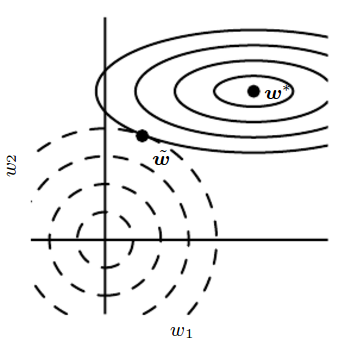
\includegraphics[width=3in]{fig/chap7/7_1.png} 
   \caption{该图描述了$L^2$(或权重衰减)正则化在最优值$w$时的影响。其中实心椭圆线条表示未加入正则化项的目标函数的等值线,虚线圈表示有着$L^2$正则化的目标函数的等值i线。在点$\widetilde{w}$处,实线条与虚线条相交达到等值。在$w_1$维度的轴线上,损失函数海森矩阵的特征值很小,当水平移动$w$使其距离$w^*$越来越远时,目标函数值并没有明显的增大。因为沿着$w_1$这个水平方向,目标函数没有表现出强烈的偏好,正则化项在这个轴线上有强作用。正则化项拉着$w_1$让它与零越来越近。在$w_2$维度上,目标函数对于$w$远离$w^*$的运动是非常敏感的,这个方向上对应的特征值很大,有着高曲率。这就导致权重衰减在$w_2$这个方向上的影响相当小。}
   \label{fig:7_1}
\end{figure}

只有能明显地减小目标函数值的参数的方向才能被相对完整保留,在不有助于减小目标函数的方向上,海森矩阵的小特征值告诉我们,在这个方向上的运动不会显着增加梯度。这种不重要方向的权向量分量通过在整个训练中使用正则化来衰减掉。

到目前为止,我们已经讨论了权重衰减在一个抽象的、一般形式以及二次的损失函数形式的优化上产生的作用。那这些作用是如何关系到机器学习中某些方面的呢?我们会发现研究线性回归(其损失函数形式是二次的)的过程也适用于我们目前使用的分析。就训练数据和当前得到的结果再次分析,我们将能够获得相同结果的特殊情况。 对于线性回归,损失函数是误差平方和的形式:
$$
\begin{aligned}
(Xw - y)^T (Xw - y).
\end{aligned}
$$
当加入$L^2$正则化项,目标函数变为:
$$
\begin{aligned}
	(Xw - y)^T (Xw - y) + \frac{1}{2} \alpha w^T w.
\end{aligned}
$$
这将会改变正规方程(normal aligneds)的解从
$$
\begin{aligned}
	w = (X^TX)^{-1}X^T y
\end{aligned}
$$
变为
$$
\begin{aligned}
	w =  (X^TX + \alpha I)^{-1}X^T y.
\end{aligned}
$$
在变化前的方程7.16中的矩阵$X^TX$是协方差矩阵$\frac{1}{m} X^T X$按照比例计算得到的,使用带$L^2$的正则项$(X^TX +\alpha I)^{-1}$替代原本的$X^TX$,最终得到上述最终变化后的方程7.17。新的到的矩阵除了在对角矩阵前加上了一个用于调节大小的超参数$\alpha$,与最初的矩阵是一样的,对角矩阵中每个元素与每个输入特征的方差一一对应。我们可以看到当输入数据的方差比较大时,$L^2$正则化可以使学习算法很好地适应输入数据$X$,它可以使得某些对应输出值较小的特征对应的权重得到一定程度的缩放(which makes it shrink the weights on features whose covariance with the output target is low compared to this added variance)。

\subsection{$L^1$参数正则化}

虽然$L^2$权重衰减是一种常见的权重衰减手段,但还有其它惩罚模型参数规模的方法。另一个选择就是$L^1$正则化方法。

严格地说,模型参数$w$的$L^1$正则化方法定义为:
$$
\begin{aligned}
	\Omega(\theta) = ||w||_1 = \sum_i |w_i|
\end{aligned}
$$
也就是每个参数的绝对值之和。我们首先会研究$L^1$正则化方法在没有偏执参数的线性回归模型上的作用,以及$L^1$与$L^2$两种正则化的不同。与$L^2$权重衰减类似,$L^1$权重衰减前面也有一个正的超参数$\alpha$用来控制惩罚权重衰减$\Omega$的力度。加入$L^1$正则后的目标函数$\widetilde{J} (w; X, y) $为:
$$
\begin{aligned}
	\widetilde{J} (w; X, y) = \alpha ||w||_1 + J(w;X,y),
\end{aligned}
$$
对应的梯度计算公式为(实际上是一个子梯度,不是完整梯度的计算形式):
$$
\begin{aligned}
\triangledown_w \widetilde{J} (w; X, y) = \alpha \text{sign} (w) + \triangledown_w J(X,y;w)
\end{aligned}
$$
其中$\text{sign}(w)$是对权重向量$w$逐个元素应用符号函数。

通过观察上面得到的最后一个方程7.20,我们可以很快发现$L^1$与$L^2$正则化有很大差别。具体而言,正则对梯度的贡献对于每个$w_i$不再是线性的;而是由一个常数因子$\alpha$和符号函数$\text{sign}(w_i)$组成。这样我们就不必要像研究$L^2$正则化时候那样仔细地研究其代数解做出一个损失函数$J(X, y; w)$的二次形式的近似。

线性模型的损失函数是二次形式的,也可以用泰勒级数表示。此外,可以想象用截断的泰勒级数这样的复杂模型来对这个损失函数进行近似,这样得到的梯度为:
$$
\begin{aligned}
	\triangledown_w \hat{J} (w) = H(w - w^*),
\end{aligned}
$$
其中,$H$是损失函数$J$关于$w$取值为$w^*$时的海森矩阵。

因为一般情况下,带上$L^1$惩罚的表达式里面还含有其它项,所以我们进一步假设得到的海森矩阵$H$是对角矩阵,即$H = \text{diag}([H_{1,1}, ..., H_{n,n}])$,其中$H$矩阵中的对角线元素$H_{i,i} > 0$。这条假设保证了线性回归问题的数据已做了去除输入特征之间的所有相关性的预处理,这个预处理过程可能是通过主成分分析完成的。

对于$L^1$正则化的目标函数的二次近似分解成一个基于参数加和的形式:
$$
\begin{aligned}
	\hat{J}(w;X,y)=J(w^*;X,y)+\sum_i\left [ \frac{1}{2} H_{i,i} (w_i - w_i^*)^2 + \alpha |w_i| \right ].
\end{aligned}
$$
最小化近似损失函数的问题有一个分析解(对每一个维度$i$),即如下形式:
$$
\begin{aligned}
	w_i = \text{sign}(w_i^*) \max\left \{ |w_i^*| - \frac{\alpha}{H_{i,i}}, 0 \right \}.
\end{aligned}
$$
考虑到所有的$i$有$w_i^* > 0$的情况,可能有两种结果:

当$w_i^* \leq \frac{\alpha}{H_{i,i}}$时,加入正则化的目标函数最优值时有$w_i = 0$。会导致这个的原因是因为$J(w; X, y)$给加入正则化后的目标函数$\widetilde{J}(w; X, y)$的贡献太大了,也就是在方向$i$上$L^1$正则化会将$w_i$的值推向零。

当$w_i^* > \frac{\alpha}{H_{i,i}}$时,正则化不会将最优值时的$w_i$移动到零,但扔会朝着相同的方向推进$\frac{\alpha}{H_{i,i}}$的距离。

当$w_i^* < 0$时,也会发生相似的过程,但$L^1$惩罚会使得$w_i$朝着正数方向移动$\frac{\alpha}{H_{i,i}}$的距离或者移动到$0$ 。

与$L^2$正则化方法相比,$L^1$正则化会产生一个更稀疏的解。在这种背景下产生稀疏解意味着某些参数计算出的解值为零。$L^1$的稀疏性与$L^2$正则化有本质上的不同,公式7.13即$\widetilde{w} = Q(\Lambda + \alpha I)^{-1} \Lambda Q^T w^*$给出了$L^2$正则化时$\widetilde{w}$的解,回顾该公式,有一个假设那就是海森矩阵$H$是对角矩阵且是正定矩阵,引入海森矩阵的目的是方便对$L^1$正则化的分析,可以发现$\widetilde{w_i} = \frac{H_{i,i}}{H_{i,i} + \alpha} w_i^*$。如果$w_i^*$是非零的,那么$\widetilde{w_i}$也是非零的。这就论证了即使 $L^1$ 在 $\alpha$ 比较大的情况下也会变为零,但 $L^2$ 正则化不会导致参数变得稀疏。

$L^1$正则化的稀疏性已被广泛用于特征选择。特征选择通过从原始的特征中选择出可用的特征子集来简化机器学习问题。特别是众所周知的LASSO(Tibshirani, 1995)(全称为:least absolute shrinkage and selection operator,即”最小绝对收缩与选择算子“)特征选择模型,它整合了$L^1$的线性模型惩罚和最小平方损失函数。$L^1$惩罚会使得权重向量中的一部分元素值变为零,这也表明这些权重所对应的特征可以被安全地舍弃掉。

在第5.6.1小节中,我们看到了很多可以理解为最大后验贝叶斯推断(MAP Bayesian inference)的正则化策略,特别是$L^2$正则化等价于有着高斯分布的先验权重的最大后验(MAP)贝叶斯推断。对于$L^1$正则化来说,当先验是各向同性拉普拉斯分布时(参见第3.26小节的方程)即$w \in \Re^n$,用于正则损失函数的惩罚项$\alpha \Omega (w) = \alpha \sum_i |w_i|$等价于由最大后验(MAP)贝叶斯推理最大化的对数先验项。
$$
\begin{aligned}
\log p(w) = \sum_i \log \text{Laplace}(w_i;0,\frac{1}{\alpha}) = -\alpha ||w||_1 + n \log \alpha - n \log2.
\end{aligned}
$$
从学习的角度来看相对$w$的最大化,我们可以忽略$\log \alpha - \log 2$这两项,因为它们的值不取决于权重$w$。

\section{约束优化的范数惩罚}

考虑参数范数惩罚的代价函数正则化:
$$
\begin{aligned}
	\widetilde{J}(\theta; X, y) = J(\theta; X, y) + \alpha \Omega(\theta).
\end{aligned}
$$
回顾4.4小节中,由于原来的目标函数有一套惩罚,通过构造一个广义的拉格朗日函数,可以使约束函数最小化。每个惩罚相当于一个乘积,乘积由两项构成:一项是被称为Karush–Kuhn–Tucker(KKT)乘子的系数,另一项是用来代表限制条件是否满足的函数。如果我们想要约束$\Omega(\theta)$小于某个常数$k$,我们可以构造一个广义拉格朗日函数:
$$
\begin{aligned}
	\mathcal{L} (\theta, \alpha; X, y) = J(\theta; X, y) + \alpha (\Omega(\theta) - k).
\end{aligned}
$$
约束问题的解由以下公式给出:
$$
\begin{aligned}
	\theta^* = \arg_{\theta} \min \max_{\alpha,\alpha \leq 0} \mathcal{L}(\theta, \alpha).
\end{aligned}
$$
正如第4.4小节所述,要计算得到$\theta^*$值需要同时修改$\theta$与$\alpha$的值,第4.5小节提供了一个带$L^2$正则化限制的线性回归的例子。许多不同的过程是可能的——某些情况可以使用梯度下降求解,而其它时候因为梯度为零而需要使用分析解,但是在所有过程中,当$\Omega (\theta) > k$时,$\alpha$必须增加,而当$\Omega (\theta) < k$时$\alpha$必须减小。所有的正值$\alpha$会促使$\Omega (\theta)$收缩,还有最佳值$\alpha^*$也会促使$\Omega (\theta)$收缩,但再怎么收缩减少也不会使$\Omega (\theta)$小于$k$。

为了进一步分析约束的作用,我们可以将$\alpha^*$的值固定并把问题变为$\theta$的函数的问题:
$$
\begin{aligned}
\theta^* = \arg_{\theta} \min \mathcal{L}(\theta, \alpha^*) = \arg_\theta \min J(\theta; X, y) + \alpha^* \Omega(\theta).
\end{aligned}
$$
这与使$\widetilde{J}$最小化的正则训练问题完全相同。因此,我们可以认为参数范数惩罚是对权重施加约束,如果$\Omega$是$L^2$范数,则权重被约束在$L^2$球中。如果$\Omega$是$L^1$范数,则权重被限制在位于有限$L^1$范数的区域中。通常我们不知道(通过使用系数$\alpha^*$的权重衰减的)约束区域的大小,因为得到了$\alpha^*$的值并不能直接得到$k$的值。原则上,可以求解这种交叉关系(fork),但是$k$和$\alpha^*$之间的关系取决于$J$的形式。虽然不知道约束区域的确切大小,但可以通过增加或减少$\alpha$来粗略地控制它,以便增长或缩小约束区域,较大的$\alpha$将导致较小的约束区域,而较小的$\alpha$将导致较大的约束区域。

有时我们可能希望使用明确的约束,而不是惩罚。如第4.4节所述,我们可以修改算法,如随机梯度下降沿$J(\theta)$下坡,然后投射$\theta$回到满足$\Omega (\theta) < k$的最近点。如果我们知道$k$的什么值是适当的并且不想花时间搜索与该$k$对应的$\alpha$值,这可能是有用的。

使用显式约束和重投影而不是用惩罚实施约束的另一个原因是惩罚可以导致非凸优化过程陷入对应于小$\theta$的局部最小值。当训练神经网络时,这通常表现为训练有几个“死掉的神经元单位”的神经网络。这些“死掉的神经元”是对网络学习的函数的行为没有多大贡献的单位,因为进入或离开这些神经元的权重都很小。当训练对权重的范数进行惩罚时,这些配置可以是局部最优的,即使可以通过使权重更大来显着减少$J$。通过重投影实现的显式约束在这些情况下的效果更好,因为这种方法不会促使权重逼近原点。通过重投影实现的显式约束只有当权重变大并且试图离开约束区域时才具有效果。

最后,使用重投影的显式约束可能是有用的,因为它们对优化过程施加了一些稳定性。当使用大学习率时,可能遇到正反馈回路,其中大的权重诱导大的梯度,然后引起对权重的大的更新。如果这些更新一致地增加权重的大小,则$\theta$迅速地从原点移开,直到出现数值溢流。具有重投影的显式约束可以防止此反馈循环,因为权重的持续增大没有限制。Hinton等人(2012c)建议使用约束结合高学习率,这样可允许快速探索参数空间,同时保持一些稳定性。

特别地,Hinton等人(2012c)推荐由Srebroand Shraibman(2005)引入的策略:约束神经网络层的权重矩阵的每列的范数,而不是约束整个权重矩阵的Frobenius范数。分别约束每列的范数可防止任何一个隐藏单元具有非常大的权重。如果我们在拉格朗日函数中将这个约束转换为惩罚,它将类似于$L^2$权重衰减,但是对于每个隐藏单元的权重具有单独的KKT乘子。这些KKT乘子中的每一个将被单独地动态地更新,以使每个隐藏单元服从约束。在实践中,列规范限制总是作为具有重投影的显式约束来实现。

\section{正则化和受约束问题}

在某些情况下,正则化对机器学习问题的正确定义是必要的。机器学习中的许多线性模型,包括线性回归和主成分分析(PCA)的计算都依赖计算翻转矩阵,即$X^T X$。$X^T X$是奇异的是不可能的(This is not possible whenever $X^T X$ is singular)。每当数据生成分布在一些方向上确实没有方差时,或者当在一些方向上没有观察到方差时,该矩阵可以是奇异矩阵,因为存在比输入的特征数目($X$的列)更少的样本数($X$的行)。在这种情况下,许多形式的正则化对应于反转$X^T X + \alpha I$,这个正则化矩阵保证是可逆的。

当相关矩阵可逆时,这些线性问题具有闭合形式解。有的问题也可能没有闭合解。一个例子是应用了逻辑回归的问题,问题中数据的类别是线性可分的。如果一个权重向量可以实现完美的分类,那么$2w$会有更大可能性实现完美分类。如随机梯度下降的迭代优化过程将不断更新$w$,并且在理论上将永远不会停止。在实践中,梯度下降的数值实现将最终使权重达到足够大引起数值溢出,此时要做的操作将取决于程序员如何处理不是实数的值。

大多数形式的正则化能够保证应用于不确定问题的迭代方法的收敛。例如,当似然性的斜率等于权重衰减系数时,权重衰减将导致梯度下降使权重不再增大。

使用正则化来解决不确定问题的想法超出了机器学习。相同的想法对于一些基本的线性代数问题也是有用的。

正如我们在2.9节中所看到的,我们可以使用Moore-Penrose伪逆来解决不确定的线性方程。回想矩阵$X$的伪逆$X^+$的定义是:
$$
\begin{aligned}
	X^+ = \lim_{\alpha \searrow 0} (X^T X + \alpha I)^{-1} X^T.
\end{aligned}
$$
我们现在可以将该上述公式7.29作为具有权重衰减的线性回归。特别地,上述公式7.29是方程7.17($w = (X^TX + \alpha I)^{-1}X^Ty$)在正则化系数收缩到零时候的极限情况。因此,我们可以将伪逆解释为使用正则化来稳定未确定的问题。

\section{数据集扩增}

使机器学习模型更好地泛化的最好方法基于更多的数据训练。当然,在实践中,我们所拥有的数据量有限。 解决这个问题的一种方法是创建假数据并将其添加到训练集,对于一些机器学习任务,创建新数据相当简单。

对于分类问题的数据扩增来说,这种方法是最容易的。分类器需要采用复杂的高维输入$x$,并用单个类别标识$y$来标记。这意味着分类器的主要任务是对于各种各样的数据变换其输出的结果是不变的。我们可以通过转换改变训练集中的$x$输入来容易地生成新的$(x, y)$样本对。

这种方法不是很容易适用于许多其他任务。例如,除非我们已经解决了密度估计问题,否则不可能为密度估计任务生成新的假数据。

对于特定分类问题,如物体识别,数据集扩增方法是一种特别有效的技术。图像是高维且包括各种变化因素的数据,其中许多因素可以容易地被模拟。即使模型采用第9章描述的卷积和池化技术具有局部平移不变性,诸如将训练图像在每个方向上平移几个像素的操作可以很大程度提升泛化性,许多其它操作,如旋转图像或缩放图像在数据扩增中也已被证明是非常有效的。

一个务必注意的是在平移的方法应用中,这种操作会对改变正确的类别。例如,光学字符识别任务需要识别'b'和'd'之间的差异以及'6'和'9'之间的差异,因此水平翻转和180°旋转不是扩增该任务数据集的适当方式。

还有一些平移方法是我们希望分类器能再见到平移后的数据预测其类别能不变的,但这些方法不容易实现。例如,平面外的旋转操作不能作为对输入像素的简单几何操作来实现。

数据集扩增对语音识别任务也有效(Jaitlyand Hinton,2013)。

在神经网络的输入中注入噪声(Sietsma和Dow,1991)也可以被看作是数据扩增的一种形式。即使小的随机噪声添加到输入,对于许多分类甚至一些回归任务仍然可以被解决。然而,神经网络证明对噪声的鲁棒不是非常好(Tang和Eliasmith,2010)。提高神经网络的鲁棒性的一种方法是简单地训练时将随机噪声加入到输入中。在输入处将噪声注入是一些无监督学习算法的一部分,如降噪自动编码器(Vincent等人,2008)。当噪声到隐藏单元时,噪声注入也起作用,这可以被看作在多个抽象级别处进行数据集增加。Poole等人(2014)最近表明,只要仔细调整噪声的幅度,这种方法就可以非常有效。Dropout是一个强大的正则化策略,将在7.12节中描述,可以看作是通过乘以噪声构建新输入的过程。

当比较机器学习基准测试结果时,考虑数据集增强的效果是很重要的。通常,手动设计的数据集扩充方案可以显着减少机器学习技术的泛化误差。为了比较一种机器学习算法与另一种机器学习算法的性能,有必要进行受控实验。当比较机器学习算法A和机器学习算法B时,有必要确保使用相同的手动设计的数据集增加方案来评估两种算法。假设与输入的许多合成变换组合时,没有数据集扩增的算法A执行得很差,而算法B执行良好。

在这种情况下,将不同的扩增变换方法进行组合可能提升模型分类性能,而不是使用机器学习算法B。有时决定一个实验是否被适当控制需要主观判断,例如将噪声引入输入的机器学习算法的数据集增加的形式。通常可应用的操作(诸如向输入添加高斯噪声)被认为是机器学习算法的一部分,而另一种是特定用在某应用领域的操作(诸如随机地剪切图像)被认为是单独的预处理步骤。

\section{噪声鲁棒性}

第7.4节提出使用对输入数据加入噪声的方法作为数据集增强策略。对于一些模型,在模型的输入处添加具有(译注:infinitesimal variance)方差的噪声等效于对权重的范数施加惩罚(Bishop,1995a,b)。在一般情况下,重要的是要记住噪声注入可以比简单地收缩参数更强大,特别是当噪声被添加到隐藏单元时。在隐藏单元处加入噪声是一个重要的话题,值得单独讨论;第7.12节中描述的dropout算法是该方法的延伸。

在正则化模型中添加噪声的另一种方式是将其添加到权重。这种技术主要用于循环神经网络(Jim等人,1996;Graves,2011)。这可以解释为对权重的贝叶斯推理的随机实现。贝叶斯学习的处理认为模型权重是不确定的,但可以通过反映这种不确定性的概率分布来表示。将噪声添加到权重是一种实用的且随机的方式来反映不确定性。

将噪声加入到权重上等同于(在一些假设下)更传统的正则化形式,从而增加要学习的函数的稳定性。考虑回归设置,其中我们希望训练使用在模型预测$\hat{y}(x)$和真实值$\hat{y}(x)$之间的最小二乘法成本函数将特征$x$的集合映射到标量的函数$y$:
$$
\begin{aligned}
J = E_{p(x,y)}[(\hat y(x) - y)^2].
\end{aligned}
$$
训练集包含$m$对标注样例$\{(x^{(1)}, y^{(1)}),\dots,(x^{(m)}, y^{(m)})\}$。

我们现在假设对于每个输入也包括网络去权重的随机扰动$\epsilon _W \sim N(\epsilon;0, \eta I )$。让我们想象一下有一个标准的$l$层多层感知机(MLP)。我们将扰动模型表示为$\hat{y}_{\epsilon_W} (x)$。除了注入噪声,我们关注的仍是最小化网络输出的平方误差。因此,目标函数变为
$$
\begin{aligned}
\tilde J_{W}
&= E_{p(x,y,\epsilon_{W})}[(\hat y_{\epsilon_{W}}(x) - y)^2] \\
&= E_{p(x,y,\epsilon_{W})}[\hat y_{\epsilon_{W}}^2(x) - 2y\hat y_{\epsilon_{W}} (x)+ y^2] .
\end{aligned}
$$
对于较小的$\eta$,对加入了权重噪声(具有协方差$\eta I$)的损失函数$J$的最小化等价于加入正则化项的$J$的最小化:$\eta E_{p(x,y)}[||\nabla_{W}~\hat y(x)||^2]$。这种形式的正则化会促使参数进入参数空间的区域,在该参数空间中,小的权重扰动对输出具有相对小的影响。换句话说,该形式会使模型处于对小权重的变化也相对敏感的区域,找到的不仅是最小值点,而且是周围被平坦区域包围的最小值点(Hochreiter和Schmidhuber,1995)。在简化的线性回归模型中(如$\hat{y}(x) = w^\top x + b$),这个正则化项为$\eta E_{p(x)}[||x||^2]$,因为不是参数的函数,因此相对于模型参数不会为损失函数$\widetilde{J}_W$贡献的梯度。

\subsubsection{在输出目标处注入噪声}

大多数数据集在$y$标签中有一些错误,当$y$错误时,对最大化$log p(y | x)$是有害的。防止这种情况的一种方法是对标签上的噪声建模。例如,假设训练集合标签$y$是以概率$1-\epsilon$正确的,其中$\epsilon$是一个小的常数,同时也意味着有$\epsilon$的概率标签$y$是错误的,当前样本标签$y$可能是其他的类型。这个假设很容易被解析地结合到成本函数中,而不是显式地采集噪声样本。

例如,标签平滑基于一个具有$k$个输出值的软性最大分类器(softmax)通过使用$\frac{\epsilon}{k-1}$和$1-\epsilon$分别替代$0$和$1$分类目标来对模型正则化。标准的交叉熵损失可以与软目标结合使用。 使用软性最大(softmax)分类器和硬目标的最大似然学习实际上可能不会收敛——软性最大(softmax)永远不能完全确认这个样本是$0$或$1$,因此它将继续学习到越来越大的权重,从而永远做出更极端的预测。可以使用其它正则化策略(如权重衰减)来防止此情况。标签平滑具有防止在不阻碍正确分类的情况下追求硬概率的优点。这个策略自从1980年代以来一直被使用,并继续在现代神经网络中突出特色(Szegedyet等人,2015)。

\section{半监督学习}

所谓半监督学习,是将$P(x)$产生的未标记样本和$P(x, y)$中的标记样本都用于估计$P(y | x)$或根据样本特征$x$来预测其类别$y$。

在深度学习的背景下,半监督学习通常指的是学习表示$h = f(x)$。目标是学习数据表征,使得来自相同类的样本具有类似的数据表征。无监督学习可以为如何在表示空间中分组的样本提供了有用的策略。在输入空间中聚集紧密的样本应能映射到相似的表示。新空间中的线性分类器在许多情况下可以实现更好的泛化(Belkin和Niyogi,2002;Chapelle等人,2003)。这种方法的一个变体是在应用分类器(在投影数据上)之前将主成分分析作为预处理步骤之一。

半监督模型中有着独立的无监督和监督的部分,它由$P(x)$或$P(x,y)$的生成模型与$P(y|x)$的判别模型组成且共享参数。我们可以对无监督或生成模型(例如$\log P(x)$或$-\log P(x,y)$)对监督模型的标准$-\log P(y | x)$进行平衡。生成模型对监督学习问题的解是一种特殊形式的先验知识(Lasserre等人,2006),即$P(x)$的结构通过某种共享参数的形式连接到$P(y | x)$的结构。通过控制生成模型中准则占总准则中的比例,可以找到比纯粹是生成模型或完全是判别模型准则进行训练得到更好的(判别与生成模型间的)平衡(Lasserre等人,2006;Larochelle和Bengio,2008)。

Salakhutdinov和Hinton(2008)描述了一种用于学习用于回归问题的核机器的核函数方法,其中使用未标记的样本来建模$P(x)$非常显着地改善了$P(y | x)$。

更多关于半监督学习的信息,请参阅Chapelle等人(2006)的文章。

\section{多任务学习}

多任务学习(Caruana,1993)是一种通过合并几个任务中产生的样本(可以被视为对参数施加的软约束)来改进泛化性能的方式。

以同样的方式,额外的训练样本对模型的参数施加更大的压力,使其更适用于一般化的值(译注:泛化能力得到提升),当模型中的一部分在多个任务之间共享时,模型的该部分被更多地约束为好的值(假设任务共享是合理的),这经常能为模型带来更好的泛化能力。

图7.2展示了一种非常常见的多任务学习形式,不同的监督任务(在给定$x$时输出预测类别$y^{(i)}$)共享相同的输入$x$,以及中间层的表示$h^{(shared)}$(多任务共享的),这些中间层的聚合因素池也是公共的(capturing a common pool of factors.)。该模型与其相关参数一般可以分为两类部分:

\begin{itemize}
\item 特定任务的参数 (只能通过各自特定任务中的样本中获得好的泛化能力),如图7.2中的上层。
\item 所有任务共享的通用参数(从所有不同任务汇集数据获得性能提升),如图7.2中的下层。
\end{itemize}

\begin{figure}[htbp] %  figure placement: here, top, bottom, or page
   \centering
   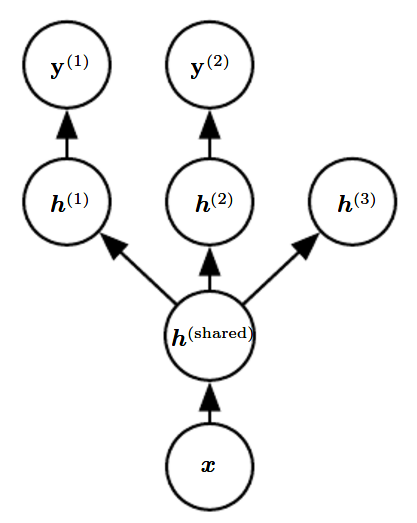
\includegraphics[width=3in]{fig/chap7/7_2.png} 
   \caption{多任务学习可以在深度学习框架中以多种方式进行,该图描述了一个通用情况,不同任务共享相同的输入但涉及不同的目标随机变量。深层网络的较低层(无论是前馈式的监督学习还是包括具有向下箭头的生成式学习)可以在不同的任务之间共享,而对于特定任务的参数(分别到达$h^{(1)}$和$h^{(2)}$的任务)可以在共享表示$h^{(shared)}$之上被学习。基本的假设是:存在解释输入$x$变化的大量共同权重因子,而每个特定任务只与这些权重因子的子集相关联。在该图的示例中,增加了假设:上层的隐藏层单元$h^{(1)}$和$h^{(2)}$专注于特定任务(分别预测$y^{(1)}$和$y^{(2)}$),而一些中间级的表示$h^{(shared)}$则在所有任务之间共享。在无监督学习中,一些上层权重与任何输出任务($h^{(3)}$)都不相关是有意义的:$h^{(3)}$相关的权重揭示了输入的变化但与预测$y^{(1)}$或$y^{(2)}$是不相关的。}
   \label{fig:7_2}
\end{figure}

因为共享参数,泛化性能得以提升并且可以得到泛化误差界限(Baxter,1995),(与单个任务相比,对于共享参数,样本数量的成比例增加)使共享参数的统计强度大大提高。当然,只有当不同任务间的统计关系的假设是有效时,某些不同任务间的参数才可以被共享使用。

从深度学习的角度来看,有如下的潜在先验知识:观察不同任务的数据变化权重,一些权重是可以在两个或多个任务之间共享的。

\section{提前终止}

因为大模型具有足够的代表能力,所以在训练大模型完成任务时,我们经常观察到随时间训练误差稳定下降,但是验证集误差开始再次上升。这个过程的示例请参见图7.3,该过程一般都会发生。

\begin{figure}[htbp] %  figure placement: here, top, bottom, or page
   \centering
   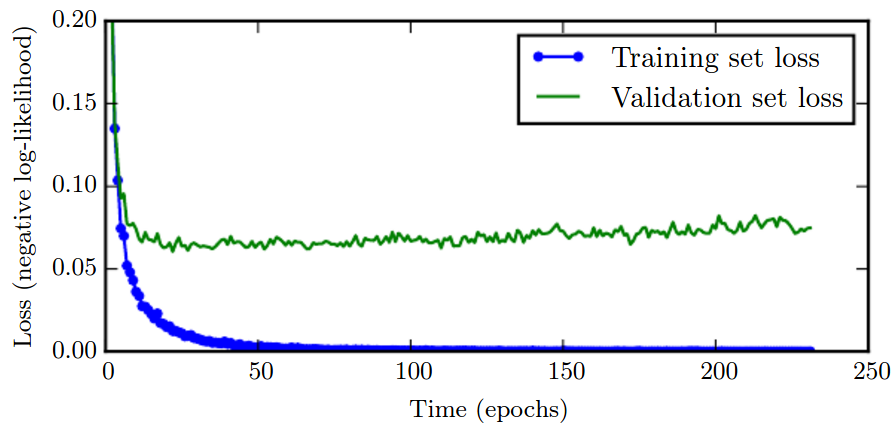
\includegraphics[width=5in]{fig/chap7/7_3.png} 
   \caption{显示负对数似然损失随时间变化的学习曲线(横坐标表示基于数据集的训练迭代次数或者一次完整的数据集遍历)。在本例中,我们在MNIST上训练一个maxout网络。观察到训练集的目标函数值随时间持续减小,但验证集平均损失函数值开始再次增加,形成不对称的U形曲线。}
   \label{fig:7_3}
\end{figure}

这意味着我们可以得到验证集误差最低时(并且很可能有更低的测试集误差)的模型。每当验证集上的误差降低时,我们便会存储此时的模型参数副本。当训练算法终止时,我们返回所有存储的模型参数,而不是最后一次的模型参数。当达到预先规定的迭代次数没有参数比最佳记录的验证误差更小时,该算法终止。这个过程在算法中有更正式的指定。

%%%%%%%%%%%%%%%%%%%%%%%%%%%%%%%%%%%%%%%%%%%%%%%%%%%%%
算法7.1用来确定最佳训练次数的提前终止(early stopping)元算法

这种元算法是一种通用策略,可以很好地与各种训练算法和验证集上的误差量化方法相结合。

令$n$为两次评估之间的步数。

令$p$为耐心程度(patience),即在算法停止前容忍算法出现更大验证集误差的次数。

令$\theta_{o}$为初始权重参数。

$\theta \leftarrow \theta_{o}$

$i \leftarrow 0$

$j \leftarrow 0$

$v \leftarrow \infty$

$\theta^* \leftarrow \theta$

$i^* \leftarrow i$

WHILE $j < p$

$\quad$运行训练算法$n$步,更新$\theta$ 。

$\quad$ $i \leftarrow i + n$

$\quad$ $v' \leftarrow \text{ValidationSetError}(\theta)$

$\quad$ IF $v' < v$

$\quad \quad j \leftarrow 0$

$\quad \quad \theta^* \leftarrow \theta$

$\quad \quad i^* \leftarrow i$

$\quad \quad v \leftarrow v'$

$\quad $ ELSE

$\quad \quad j \leftarrow j + 1$

$\quad$ ENDIF

ENDWHILE

最佳参数为$theta^*$,最佳训练步数为$i^*$
%%%%%%%%%%%%%%%%%%%%%%%%%%%%%%%%%%%%%%%%%%%%%%%%%%%%%

这种策略被称为提前终止。它可能是深度学习中最常用的正则化形式,该方法的普及是因为有效和简单。

提前终止(early stopping)可以被认为是非常高效的超参数选择算法。在这一个观点下,训练步数只是另一个超参数。可以在图7.3中看到,这个超参数具有U形验证集的性能曲线。大多数控制模型能力的超参数都具有如图5.3所示的U形验证集性能曲线。在使用提起终止(early stopping)的情况下,通过确定对训练集拟合所需的训练步数来控制模型能力。大多数超参数选择所需的计算和检查的代价都很大,在训练开始时设置超参数,然后运行几步训练查看效果。“训练时间”(training time)超参数是唯一的,因为它定义了训练所需的时间,并在此训练过程中尝试了其他超参数的许多值。通过提前终止(early stopping)自动选择此超参数的唯一需要的是在训练期间定期对验证集评估。理想情况下,这个过程是在单独机器,或单独CPU或单独GPU上进行的,与训练过程并行完成。如果没有这么多计算资源,则可以使用比训练集小的验证集验证,或减少评估验证集误差的次数,来获得最佳训练时间的大致估计来降低周期性估计超参数带来的成本。

提前终止(early stopping)还要做的保存一份当前得到的最佳参数的副本。该操作通常可以忽略,因为可以将这些参数存储在较慢和较大形式的存储器中(例如,在GPU存储器中训练,在主机存储器或磁盘驱动器中存储训练得到的最佳参数)。由于最佳参数很少写入并且在训练期间从不读取,所以这些偶尔的慢写入对总训练时间几乎没有影响。

提前终止(early stopping)是一种非常不明显的正则化形式,因为它对训练中的目标函数或参数空间的值的集合几乎没有改变。这意味着在不损害学习的动态过程中,提前终止(early stopping)是易于使用的。这与权重衰减形成对比,必须注意不要使用太大的权重衰减,因为这回导致网络陷入陷入不好的局部最小值,对应得到不正确的小值权重。

提前终止(early stopping)可以单独使用或与其它正则化策略结合使用。即使通过修正目标函数的方法以促进更好的泛化性能的正则化策略时,最好的泛化表现很少出现在训练目标函数的局部最小值处。

提起终止(early stopping)需要一个验证集,这意味着有一些训练数据不会用于模型训练。为了能最好地利用这一额外的数据,其一是可以在初始训练与提前终止完成之后执行额外的训练。在第二个额外训练步骤中,包括所有训练数据。有两个基本策略可以用于该第二训练过程。

一个策略(算法7.2)是再次初始化模型并基于所有数据重新训练。在第二次训练中,我们训练使用第一次训练中提前停止确定的最佳的迭代次数。在此过程中有一些细节,例如,没有一种好的方式来知道是否基于数据集重新训练相同数量的参数更新,或相同数量的传播。在第二轮训练中,每次通过数据集将需要更多的参数更新,因为训练集更大。

%%%%%%%%%%%%%%%%%%%%%%%%%%%%%%%%%%%%%%%%%%%%%%%%%%%%%
算法7.2

使用提前终止(early stopping)确定训练步数,之后在所有数据重新训练的元算法。

$X^{(train)}$和$y^{(train)}$是训练集。

将训练集$X^{(train)}$和$y^{(train)}$分别切分成$(X^{(subtrain)}, X^{(valid)})$和$(y^{(subtrain)}, y^{(valid)})$。

执行提前终止(算法7.1),随机初始化$\theta$,使用训练数据集$(X^{(subtrain)}, y^{subtrain})$以及验证数据集$X^{(valid)}$和$y^{(valid)}$。将返回$i^*$,即最佳的迭代次数。

再次对$\theta$随机初始化。


基于训练数据集$X^{train}$和$y^{(train)}$迭代$i^*$次。
%%%%%%%%%%%%%%%%%%%%%%%%%%%%%%%%%%%%%%%%%%%%%%%%%%%%%

另一个基于所有数据的策略是保持从第一轮训练中获得的参数,然后继续训练,但现在使用所有数据。在该阶段已经不再有一个何时哪次迭代停止的引导。相反,可以监视验证集上的平均损失函数,并继续训练直到它低于训练集目标函数的值,在该值处执行提前终止(early stopping)。这种策略避免了从头开始重新训练模型的高成本,但是表现并不是很好。例如,无法保证验证集的目标函数值将达到目标值,该策略甚至不能保证终止。这个过程在算法7.3中有更正式地描述。

提前终止(early stopping)也是有用的,因为它减少了训练过程的计算成本。除了由于限制训练迭代次数而明显降低计算成本之外,它还具有提供正则化的好处,而不需要在成本函数或附加项的梯度的计算中添加惩罚项。

\textbf{如何让提前终止(early stopping)发挥正则化的作用}:迄今为止,我们已经说过提前终止(early stopping)是一个正则化策略,但支持该说法的只有通过绘制出验证集误差的U型学习曲线。提前终止规范模型的实际机制是什么?Bishop(1995a)、Sjöberg和Ljung(1995)认为提前终止(early stopping)具有将优化过程限制在初始参数值$\theta$附近相对小范围参数空间的效果,如图7.4所示。具体而言,假设经过$\tau$步优化(训练迭代的次数)和使用学习速率$\epsilon$。我们可以将这二者乘积$\epsilon \tau$作为模型能力(effective capacity)的一种度量。假设梯度值是有范围限制的,那么限制迭代次数和学习速率将会限制从$\theta_0$可达到的参数空间的范围。那么可以说,$\tau$起到了权重衰减系数的倒数(reciprocal of the coefficient used for weight decay)的作用。

%%%%%%%%%%%%%%%%%%%%%%%%%%%%%%%%%%%%%%%%%%%%%%%%%%%%%
算法7.3

元算法在目标函数(即损失函数)值即将过拟合时候使用提前终止(early stopping)策略,直到目标函数值开始过拟合时之后继续训练。

$X^{(train)}$和$y^{(train)}$是训练集。

将训练集$X^{(train)}$和$y^{(train)}$分别切分成$(X^{(subtrain)}, X^{(valid)})$和$(y^{(subtrain)}, y^{(valid)})$。

执行提前终止(算法7.1),随机初始化$\theta$,使用训练数据集$(X^{(subtrain)}, y^{subtrain})$以及验证数据集$X^{(valid)}$和$y^{(valid)}$。这将会对$\theta$进行更新。

$\epsilon \leftarrow J(\theta, X^{(subtrain)}, y^{(subtrain)})$当(while)$J(\theta, X^{(valid)}, y^{(valid)}) > \epsilon$时,$\quad$基于$X^{(train)}, y^{(train)}$训练$n$步迭代,

结束(while)循环。
%%%%%%%%%%%%%%%%%%%%%%%%%%%%%%%%%%%%%%%%%%%%%%%%%%%%%

事实上,我们可以展示如何在具有二次的损失函数和梯度下降的线性模型的情况下,提前终止(early stopping)等价于$L^2$正则化。

为了与经典的$L^2$正则化比较,我们做出一个简单的设定,其中只有参数是线性权重(即$\theta = w$)。我们可以使用在权重$w^*$为最佳值的邻域中的二次近似来建模成本函数$J$:
$$
\begin{aligned}
\hat{J} (\theta) = J(w^*) + \frac{1}{2} (w - w^*)^T H(w - w^*),
\end{aligned}
$$
其中,$H$是损失函数$J$在权重参数$w$取值为$w^*$时的海森矩阵。假设$w^*$是损失函数$J(w)$最小值时的取值,我们知道$H$是半正定矩阵。在局部泰勒级数近似(local Taylor series approximation)下,给出如下梯度的计算公式:
$$
\begin{aligned}
\triangledown_w \hat{J}(w) = H(w - w^*).
\end{aligned}
$$
\begin{figure}[htbp] %  figure placement: here, top, bottom, or page
   \centering
   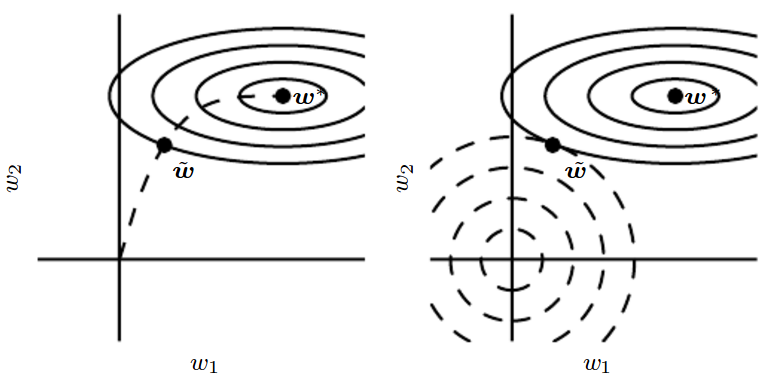
\includegraphics[width=5in]{fig/chap7/7_4.png} 
   \caption{提起终止(early stopping)的图像描绘。(左)图中的实线等高线表示负对数似然(negative log-likelihood)的轮廓,短划线则是随机梯度下降从起始点开始的轨迹线。最终算法停止的位置不在损失函数最小值对应权重参数$w^*$的位置处,提前终止(early stopping)会使轨迹线早于损失函数最小值对应的$w^*$处停下。(右)图是用于和$L^2$正则效果比较的图示,虚线圈表示$L^2$正则的等高线,$L^2$正则会使总损失函数的最小值比未正则化的损失函数的最小值更靠近原点。}
   \label{fig:7_4}
\end{figure}

我们将在训练期间研究参数向量遵循的轨迹。为简单起见,将初始参数向量设置为原点(对与神经网络而言,为了获得隐含单元间的对称破碎(symmetry breaking),如第6.2小节描述的,不能设定初始时的权重参数都为$0$。但该论点适用于其它任何初始值$w^{(0)}$),即$w^{(0)}=0$。让我们通过分析$\hat{J}$上的梯度下降来研究与$J$上梯度下降的近似行为:
$$
\begin{aligned}
w^{(\tau)} & = w^{(\tau - 1)} - \epsilon \bigtriangledown_w \hat{J} (w^{(\tau - 1)}) \\
& = w^{(\tau - 1)} - \epsilon H (w^{(\tau - 1)} - w^*) \\
w^{(\tau)} - w^* & = (I - \epsilon H)(w^{(\tau - 1)} - w^*).
\end{aligned}
$$
让我们现在在$H$的特征向量的空间中重写这个表达式,利用$H$的特征分解:$H = Q \Lambda Q^T$,其中$\Lambda$是对角矩阵,$Q$是特征向量的正交基。
$$
\begin{aligned}
w^{(\tau)} - w^* & = (I - \epsilon Q \Lambda Q^T) (w^{(\tau - 1)} - w^*) \\
Q^T (w^{(\tau)} - w^*) & = (I - \epsilon \Lambda ) Q^T (w^{(\tau - 1)} - w^*)
\end{aligned}
$$
假设$w^{(0)} = 0$同时$\epsilon$选择一个足够小的保证$|1 - \epsilon \lambda_i| < 1$成立的值。$\tau$参数更新后训练的参数轨迹如下:
$$
\begin{aligned}
	Q^T w^{(\tau)} = [I - (I - \epsilon \Lambda)^{\tau}] Q^T w^*.
\end{aligned}
$$
现在,用于$L^2$正则化的等式7.13(即$\widetilde{w} = Q(\Lambda + \alpha I)^{-1} \Lambda Q^T w^*.$)中的$Q^T\widetilde{w}$的表达式可以后推为:
$$
\begin{aligned}
Q^T \widetilde{w} & = (\Lambda + \alpha I)^{-1} \Lambda Q^T w^* \\
Q^T \widetilde{w} & = [I - (\Lambda + \alpha I)^{-1} \alpha] Q^T w^*
\end{aligned}
$$
比较方程7.40($Q^T w^{(\tau)} = [I - (I - \epsilon \Lambda)^{\tau}] Q^T w^*$)与7.42($Q^T \widetilde{w} = [I - (\Lambda + \alpha I)^{-1} \alpha] Q^T w^*$),如果选择超参数$\epsilon, \alpha, \tau$,那么有:
$$
\begin{aligned}
	(I - \epsilon \Lambda)^{\tau} = (\Lambda + \alpha I)^{-1} \alpha,
\end{aligned}
$$
那么可以看出$L^2$正则化和提前终止(early stopping)是等价的(至少在目标函数的二次近似下)。进一步讲,通过采用对数和使用对数$\log{(1+x)}$的序列展开,可以得出结论:当所有$\lambda_i$都很小时(即$\epsilon \lambda_i \ll 1\ and\ \lambda_i/\alpha \ll 1$),那么
$$
\begin{aligned}
\tau \approx \frac{1}{\epsilon \alpha}, \\
\alpha \approx \frac{1}{\tau \epsilon}.
\end{aligned}
$$
也就是说,在这些假设下,训练迭代次数$\tau$与$L^2$正则化参数成反比,$\tau \epsilon$具有权重衰减系数倒数的作用。

对应于(目标函数的)曲率显著方向的参数值被正则化为小于较小曲率的方向。当然,在提前终止(early stopping)中,这实际上对应于曲率显著变化方向的参数倾向学习较小曲率方向的参数(this really means that parameters that correspond to directions of significant curvature tend to learn early relative to parameters corresponding to directions of less curvature.)。

本节中的推导已经表明,长度为$\tau$的轨迹在对应于$L^2$正则化目标的最小值的点处结束。提前终止(early stopping)当然不仅仅是对轨迹长度的限制;相反,提前终止(early stopping)通常涉及监测验证集误差,以便在空间中特别好的点处停止轨迹。因此,提前终止(early stopping)具有的优点要超过权重衰减,即提前终止(early stopping)自动地确定正则化的正确量,然而权重衰减需要做很多不同的超参数取值时的训练实验。

\section{参数绑定与参数共享}

本章到目前为止,当讨论给参数加入限制或惩罚时,我们总是限定在固定的区域或点中。例如,$L^2$正则化(或权重衰减)惩罚模型参数从参数的固定值零的偏离开始。然而,有时可能需要另外能表达关于模型参数合适值的先验知识。有时可能不知道参数应该采用什么值,但是知道从领域和模型架构的知识,这其中应该有一些模型参数之间的依赖关系。

我们经常想要表达的常见类型的依赖性是某些参数应当彼此接近。考虑以下情况:我们有两个模型执行相同的分类任务(具有相同的类集合),但具有稍微不同的输入数据分布。正式地,我们有参数$w^{(A)}$的模型A和具有参数$w^{(B)}$的模型B,两个模型将输入映射到两个不同但相关的输出:$\hat{y}^{(A)} = f(w^{(A)}, x)$和$\hat{y}^{(B)} = g(w^{(B)}, x)$。

让我们假设任务是相似的(可能具有类似的输入和输出分布),我们认为模型参数应该彼此接近:$\forall i, w_i^{(A)}$应该接近$w_i^{(B)}$。我们可以通过正则化利用这些信息。具体来说,可以使用以下形式的参数规范惩罚:$\Omega (w^{(A)}, w^{(B)}) = || w^{(A)} - w^{(B)} ||_2^{2}$。这里我们使用了$L^2$惩罚,但其它选择也是可能的。

这种方法是由Lasserre等人(2006)提出,将一个模型的参数正则化,使用监督学习的范式训练为分类器,接近另一个使用无监督范式(捕获观察输入数据的分布)训练的模型的参数。构造体系结构使得分类器模型中的许多参数可以与无监督模型中的相应参数配对。

虽然参数范数惩罚是将参数正则化为(译注:让二者模型)彼此接近的一种方式,但更常用的方式是使用约束:迫使参数集相等,这种正则化方法通常被称为参数共享(parameter sharing),因为我们将各种模型或模型组件解释为共享所有参数集合中的其中一组唯一的参数。参数共享在正则化上要关闭的参数(通过范数惩罚)的显着优点(A significant advantage of parameter sharing over regularizing the parameters to be close (via a norm penalty))是只需要将所有权重参数(中唯一集合)的子集存储在存储器中,在某些模型中如卷积神经网络,参数共享可以使模型的内存占用显着减少。

\subsubsection{卷积神经网络}

到目前为止,使用最流行且最被广泛使用的参数共享是应用于计算机视觉的卷积神经网络(CNNs)。

自然图像具有对于平移不变等的许多统计特性。例如,如果猫的照片向右平移一个像素,则猫的照片仍然是猫的照片。卷积神经网络通过在图像上多个位置共享参数来考虑此属性。在输入中的不同位置计算相同的特征(具有相同权重的隐含单元)。这意味着我们可以使用相同的猫检测器找到猫,无论猫出现在图像中的第$i$列还是第$i + 1$列。

参数共享可使卷积神经网络显著减少模型参数的数量,并在不需要增加训练数据的前提下可显著增加网络规模(译注:深度或宽度)。参数共享策略仍然是将领域知识考虑到网络架构中的最好案例之一。

卷积神经网络的更多细节将在第9章讨论。

\section{稀疏表示}

权重衰减通过直接对模型参数施加惩罚来起作用。另一个策略是在神经网络中的单元激活施加惩罚,鼓励它们的激活变得稀疏的。这间接地对模型参数施加了复杂的惩罚。

我们已经讨论了(在7.1.2节中)$L^1$惩罚如何诱导稀疏参数化——这意味着许多参数变为零(或接近零)。另一方面,表示稀疏性描述了一种数据表示,这是一种许多元素为零(或接近零)的表示。这种区别的简化表示可以在线性回归中描述为:
$$
\begin{aligned}
\underset{y ~\in~ \Re^m}{
\begin{bmatrix}
18 \\ 5 \\ 15 \\ -9 \\ -3
\end{bmatrix}} =
\underset{A ~\in~ \Re^{m \times n}}{
\begin{bmatrix}
4 & 0 & 0 & -2 & 0 & 0 \\
0 & 0 & -1 & 0 & 3 & 0 \\
0 & 5 & 0 & 0 & 0 & 0 \\
1 & 0 & 0 & -1 & 0 & -4 \\
1 & 0 & 0 & 0 & -5 & 0
\end{bmatrix}}
\underset{x ~\in~ \Re^n}{
\begin{bmatrix}
2 \\ 3\\ -2\\ -5 \\ 1 \\ 4
\end{bmatrix} }\\
\underset{y ~\in~ \Re^m}{
\begin{bmatrix}
-14 \\ 1 \\ 19 \\ 2 \\ 23
\end{bmatrix}} =
\underset{B ~\in~ \Re^{m \times n}}{
\begin{bmatrix}
3 & -1 & 2 & -5 & 4 & 1 \\
4 & 2 & -3 & -1 & 1 & 3 \\
-1 & 5 & 4 & 2 & -3 & -2 \\
3 & 1 & 2 & -3 & 0 & -3 \\
-5 & 4 & -2 & 2 & -5 & -1
\end{bmatrix}}
\underset{h \in \Re^n}{
\begin{bmatrix}
0 \\ 2 \\ 0 \\ 0 \\ -3 \\ 0
\end{bmatrix} }
\end{aligned}
$$
在第一个表达式中,我们有一个稀疏参数化线性回归模型的例子。在第二个中,我们使用数据$x$的稀疏表示$h$进行线性回归。 也就是说$h$是$x$的函数,在某种意义上,$x$表示存在于$x$中的信息,但是使用稀疏向量。

表示正则化通过我们在参数正则化中使用的相同种类的机制来完成。

通过向损失函数$J$添加对表示的规范惩罚来执行表示的规范惩罚正规化。该惩罚被表示为$\Omega$。如前所述,我们用$\widetilde{J}$表示正则化损失函数:
$$
\begin{aligned}
	\widetilde{J} (\theta; X, y) = J(\theta; X, y) + \alpha \Omega (h)
\end{aligned}
$$
其中$\alpha \in [0, \infty)$表示加权范数惩罚项的相对贡献,较大的$\alpha$值对应于正则化项的加强。

正如参数上的$L^1$正则诱发参数稀疏性一样,对表示元素上的$L^1$正则也会引起表示稀疏性:$\Omega (h) = ||h||_1 = \sum_i |h_i|$。当然,$L^1$正则只是可以导致稀疏表示的正则方法的一个选择。其他的包括来自学生提出的正则(Olshausen和Field,1996;Bergstra,2011)和KL散度正则(Larochelle和Bengio,2008),对元素被限制在单元间隔的情形特别有用。Lee等人(2008)和Goodfellow等人(2009)都提出了基于几个样本$\frac{1}{m} \sum_i h^{(i)}$的平均激活进行正则化,让其接近某个目标值的策略,例如每个元素都为$0.01$的向量。

其他方法获得具有对激活值的硬约束的表示稀疏性。 例如,正交匹配追踪(orthogonal matching pursuit,Pati等人,1993)用表示h对输入x进行编码,来解决约束优化问题。
$$
\begin{aligned}
	\arg_{h, ||h||_0 < k} \min ||x - Wh||^2,
\end{aligned}
$$
其中$||h||_0$是$h$中非零项的数目。当$W$被约束为正交时,这个问题可以被有效解决。此方法通常称为OMP-k,$k$值为允许的非零特征的数量。Coates和Ng(2011)证明OMP-1可以是深层架构非常有效的特征提取器。

基本上任何具有隐藏单元的模型都可以被稀疏化。在本书中,我们将看到许多在各种情景中使用稀疏正则化的例子。

\section{Bagging和其它集成方法}

Bagging(bootstrap aggregating的简写)是一种通过组合几个模型来减少泛化误差的技术(Breiman,1994)。想法是分别训练几个不同的模型,然后让所有的模型投票输出测试示例的预测结果。 这是在机器学习称为模型平均的策略。采用这种策略的技术被称为集成方法(ensemble methods)。

模型平均能够有效的原因是不同的模型通常不会在测试集上的所有样本上产生相同的错误。

考虑一个集成$k$个回归模型的例子。假设每个模型在每个样本上的误差是$\epsilon_i$,误差服从零均值,方差为$E[\epsilon_i^2] = v$且协方差为$E[\epsilon_i \epsilon_j] = c$的多维正态分布。基于所有模型得到的集成模型的平均预测误差是$\frac{1}{k} \sum_i \epsilon_i$。集成模型得到的预测器平方误差的期望是

$$
\begin{aligned}
E \Bigg[\Bigg(\frac{1}{k} \sum_i \epsilon_i \Bigg)^2\Bigg]
& = \frac{1}{k^2} E \Bigg[\sum_i \Bigg(\epsilon_i^2 + \sum_{j \neq i} \epsilon_i \epsilon_j\Bigg)\Bigg], \\
& = \frac{1}{k} v + \frac{k-1}{k} c .
\end{aligned}
$$

在误差完全相关且$c = v$的情况下,均方误差减小到$v$,因此模型平均根本不起作用。在误差完全不相关并且$c = 0$的情况下,集成的预期平方误差仅为$\frac{1}{k}v$。这意味着模型集成的预期平方误差随集成模型的模型数目而线性减小。换句话说,平均而言,集成模型的表现将至少与其所有模型中的任何一个一样好,并且因为每个模型有各自的误差,集合模型相比成员模型的表现得到显著的改善。

不同的集成方法以不同的方式构建模型集成。例如,集成的每个成员模型可以通过使用不同的算法或目标函数训练完全不同种类的模型来形成集成。Bagging是一种允许相同类型的模型、训练算法和目标函数被重复使用多次的方法。

\begin{figure}[htbp] %  figure placement: here, top, bottom, or page
   \centering
   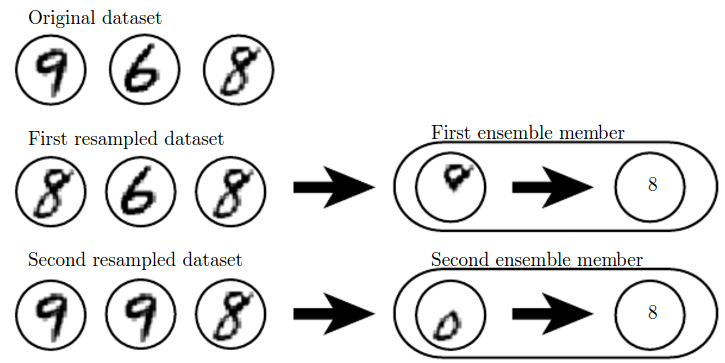
\includegraphics[width=5in]{fig/chap7/7_5.png} 
   \caption{该图是bagging如何工作的卡通描述。假设在上面描述的数据集上训练一个数字8检测器,原始数据集包含数字8、6和9。假设我们做出两个不同的重采样数据集。Bagging训练过程是用替换抽样来构造数据集中的每个样本。第一个数据集忽略掉数字9的数据并用数字8替换。在此数据集上,检测器获知数字顶部的圈对应于8的部分。在第二个数据集上,我们用数字9的数据来替换数字6的数据。在这种情况下,检测器获知数字底部的小圈对应于数字8的部分。每个单独的分类规则是脆弱的,但是如果平均它们的输出,则检测器是鲁棒的,只有当数字8的两个圈同时存在时才实现最大的置信度。}
   \label{fig:7_5}
\end{figure}

具体来说,bagging涉及构建$k$个不同的数据集。每个数据具有与原始数据集相同数量的样本,但每个数据集是通过从原始数据集中替换进行抽样构建的。这意味着有很大概率下,每个数据集都是原始数据集的一个子集,并且(如果在训练集中每次抽样原始数据集约$\frac{2}{3}$样本)还包含若干(译注:与先前抽样得到的数据集)重复的样本。模型$i$基于数据集$i$训练。每个数据集中包括的样本之间的差异导致训练模型之间的差异。参见图7.5的例子。

神经网络被广泛地用在各种解决方案中,即使所有的模型在同一个数据集上训练,他们通常也可从模型平均中获益。随机权重初始化,随机选择小样本批量,超参数的差异或神经网络的非确定性实现的不同结果的差异,通常足以导致集成所采用的不同模型成员产生部分独立的错误。

模型平均是一种用于减少泛化误差的强大且可靠的方法。科学论文的基准算法通常不鼓励使用它,因为任何机器学习算法都可以增加计算和内存为代价从模型平均中获益。因此,基准通常使用单个模型。

机器学习竞赛中常用的策略就是通过使用在数十个模型上的模型平均的方法来获得结果。最近一个突出的例子是Netflix大奖赛中的第一名所使用的模型集成策略(Koren,2009)。

不是所有用于构建集成的技术可使集成后的模型比单个模型更加具有正则化(译注:意味着更低的泛化误差)。例如,称为boosting的技术(Freund和Schapire,1996b,a)可构建具有比单个模型更高容量的集成模型。Boosting已经应用于构建多个神经网络的集成(Schwenk和Bengio,1998),通过向集成模型中增量地添加不同的神经网络。Boosting也被应用于将单个神经网络解释为一个集成模型(Bengio等人,2006a),模型成员是在该单个神经网络逐步添加隐藏单元向一个完整神经网络构建的过程中形成的。

\section{Dropout}

Dropout(Srivastava等人,2014)是一种计算量不大但功能强大的方法,可用来正则一大类模型。第一种近似下,dropout可以被认为是一个方法,使许多大型神经网络能够集成的更实用的Bagging方法。Bagging涉及训练多个模型,并在每个测试样本上评估多个模型。当每个模型是大型神经网络时就不切实际了,因为训练和评估这样的网络在运行时间和所需内存方面的代价大。通常使用五到十个神经网络集成——Szegedy等人(2014a)使用六个神经网络赢得ILSVRC比赛,但超过这个数目会使集成的结果迅速变得笨拙。即使是对指数级数目的神经网络做集成,dropout也是一种低成本的近似训练和评估一个bagged的集成模型的方法。

特别地,dropout训练由所有子网络组成的整体,如图7.6所示,这个整体中的子网络每个可以通过从原本的基础网络中去除某些非输出单元形成。在大多数现代神经网络中,基于一系列的变换和非线性操作,我们可以通过将其输出值乘以零来从网络中有效地移除该单元。该过程需要对模型进行一些轻微修改,如径向基函数网络中网络单元的状态和一些参考值。在这里为简单起见,我们提出了以零乘法为基础的dropout算法,但是它可以被简单地与网络中移除单元的其它操作一起工作。

回想一下,用bagging学习,我们定义k个不同的模型,通过从具有替换的训练集中抽样构建$k$个不同的数据集,然后在数据集$i$上训练模型$i$。Dropout的目的是近似这个过程,而不是构造指数数量规模的神经网络。具体来说,为了借助dropout进行训练,我们使用一个基于小批量样本的学习算法,每次更新是小步骤的,好比随机梯度下降。每次将一个样本加载到一个小批量样本中,我们随机抽样一个不同的二进制掩码,以应用于网络中的所有输入和隐藏单元。每个单元的掩码独立于所有其它单元进行采样。采样掩码值为$1$的概率(也导致一个单元会被包括进去)是在训练开始之前就被确定的超参数。它不是当前模型参数或输入样本的函数。通常以$0.8$的概率包括输入单元,以$0.5$概率包括隐含单元。然后我们照常运行正向、反向传播和学习更新。图7.7说明了如何使用dropout运行正向传播。

更正式地说,假设有掩码向量$\mu$其每个元素为指定包含的单元,并且$J(\theta, \mu)$定义了模型的损失,参数$\theta$和掩码$\mu$定义了模型。dropout训练包括最小化$E_{\mu} J(\theta, \mu)$。期望包含指数个项,但是我们可以通过对掩码向量$\mu$的采样值获得其梯度的无偏估计。

Dropout训练与bagging训练不完全相同。在bagging策略下,模型都是独立的。在dropout策略下,模型共享参数,每个模型继承来自父神经网络参数的不同子集。该参数共享使得用少量的内存就可以表示指数数量的模型。在bagging策略下,每个模型的训练都会收敛其相应的训练集。在dropout策略下,通常大多数模型没有被明确训练——通常当模型足够大时,若有足够多的时间,采样所有可能的子网络是可行的。相反,单步更新是基于采样到的子网络的训练,并且参数共享使得剩余子网络的参数达到较好值。这些是dropout和bagging的唯一区别。除此之外,dropout与bagging算法一致。例如,每个子网络的训练集合是用替换采样原始训练集合的方法得到的子集。

\begin{figure}[htbp] %  figure placement: here, top, bottom, or page
   \centering
   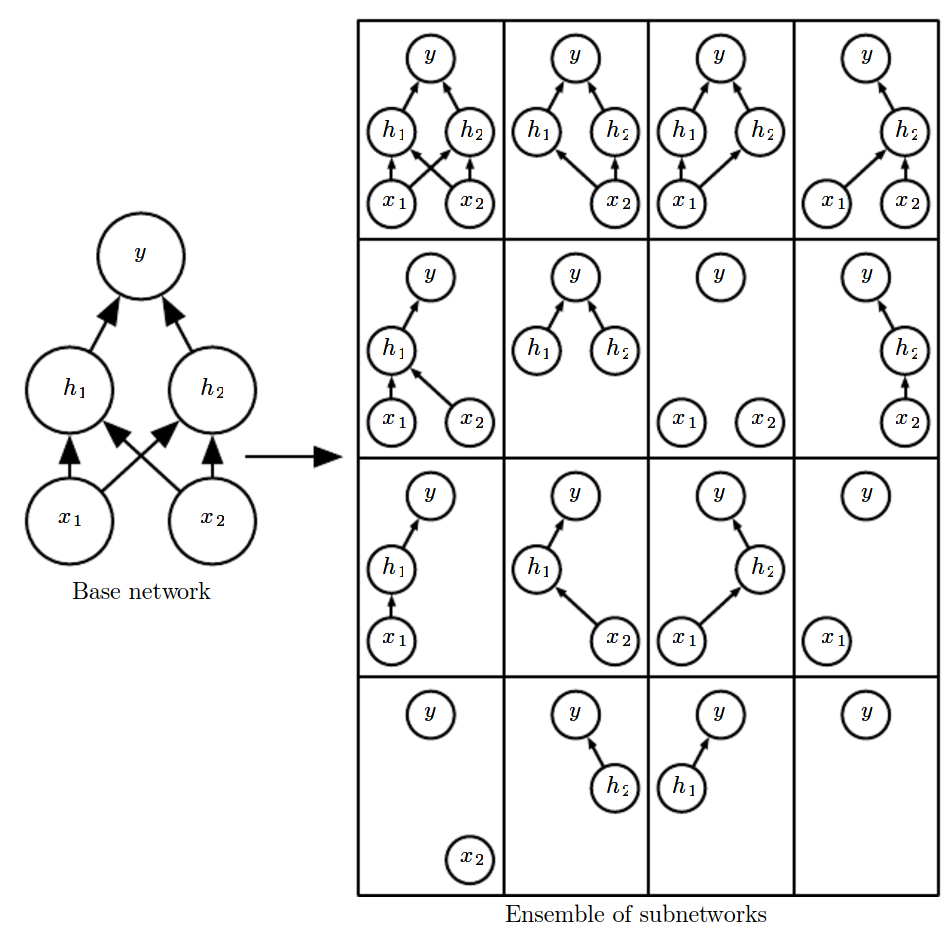
\includegraphics[width=5in]{fig/chap7/7_6.png} 
   \caption{dropout的训练基于所有子网络组成的集成,可以通过从底层基础网络中删除非输出单元后得到的网络来构建。这里,我们从具有两个可见单元和两个隐含单元的基本网络开始。这四个单元有十六中可能的网络子集。改图展示了从原始网络中丢弃不同的单元子集而形成的所有十六个子网络。在这个小例子中,所得到的网络的大部分没有输入单元或没有将输入连接到输出的路径。这个问题相比具有较宽层的网络变得不重要,丢弃从输入到输出的所有可能路径的对较宽层网络的概率更低。}
   \label{fig:7_6}
\end{figure}

\begin{figure}[htbp] %  figure placement: here, top, bottom, or page
   \centering
   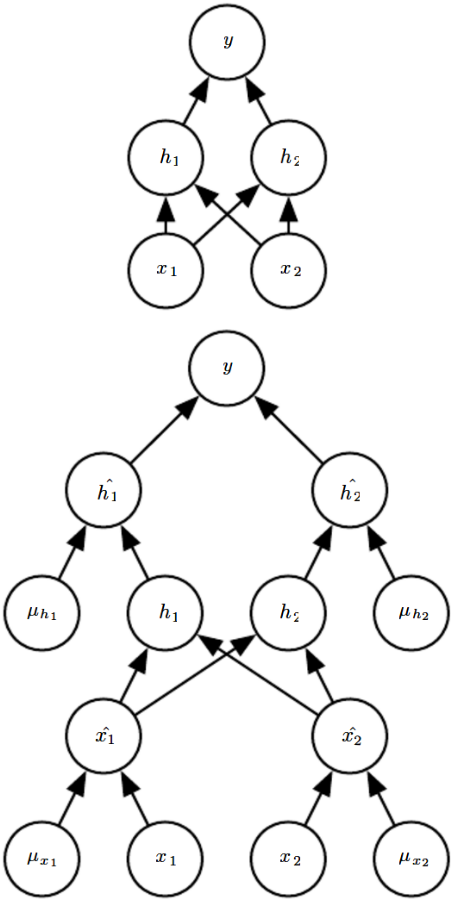
\includegraphics[width=3in]{fig/chap7/7_7.png} 
   \caption{使用dropout策略下网络正向传播的示例。(在上图中)有两个输入单元,一个隐藏层和两个隐藏单元以及一个输出单元的前馈网络。(在下图中)是dropout策略下的正向传播,对于网络中的每个输入或隐藏单元,随机抽取矢量$\mu$中的一个元素。$\mu$的元素都是二进制的,并且彼此独立地采样。每个元素为$1$的概率是超参数,对于隐藏层该超参数通常为$0.5$,而输入层通常为$0.8$。网络中的每个单元乘以相应的掩码,然后正常传播继续通过网络的其余部分。这相当于从图7.6中随机选择一个子网络,并向前传播。}
   \label{fig:7_7}
\end{figure}

为了做出预测,一个bagging策略的集成模型的结果必须依赖所有成员的累积投票。我们将这个过程称为推断。到目前为止,我们对bagging和dropout的描述不需要模型明确的概率。现在,我们假设模型的作用是输出概率分布。 在装袋的情况下,每个模型$i$产生概率分布$p^{(i)} (y|x)$。整体的预测由所有这些分布的算术平均值给出,
$$
\begin{aligned}
	\frac{1}{k} \sum_{i=1}^{k} p^{(i)} (y | x).
\end{aligned}
$$
在dropout策略下,由掩码向量$\mu$定义的每个子模型,每个自模型定义概率分布$p(y | x, \mu)$。所有掩码的算术平均值由下式给出
$$
\begin{aligned}
	\sum_{\mu} p(\mu) p(y|x,\mu)
\end{aligned}
$$
其中$p(\mu)$是用于在训练时间采样$\mu$的概率分布。

因为这个加和包括指数数目的项,除非模型结构允许某种形式简化的情况下,否则难以评估。到目前为止,深层神经网不允许任何易于理解的简化。相反,我们可以用抽样来近似推理,通过对许多掩码的输出求平均来近似。即使是10-20个掩码,通常也足以获得良好的性能。

然而有一个更好的方法,能够仅以一个前向传播的代价获得整个集成模型预测的良好近似。为此,在集成模型成员的预测分布上我们从几何平均数改用算术平均数。Warde-Farley等人(2014)提出的论点和实证证据表明在这种情况下几何平均值与算术平均值等价。

多个概率分布的几何平均值不能保证为概率分布。为了保证结果是一个概率分布,我们强加的要求是,没有一个子模型将概率$0$分配给任何事件,并且我们对结果分布进行重新归一化。由几何平均直接定义的非规格化概率分布(unnormalized probability distribution)由下式给出
$$
\begin{aligned}
\tilde{p}_{\text{ensemble}}(y \mid x) = \sqrt[2^d]{\prod_{\mu} p(y \mid x, \mu)},
\end{aligned}
$$
其中$d$是可以丢弃的单元数。这里我们使用均匀分布$\mu$来简化表示,但非均匀分布也是可能的。为了做出预测,我们必须重新标准化集成模型(re-normalize the ensemble):
$$
\begin{aligned}
p_{\text{ensemble}}(y \mid x) = \frac{\tilde{p}_{\text{ensemble}}(y \mid x)}
{\sum_{y'}\tilde{p}_{\text{ensemble}}(y' \mid x) }.
\end{aligned}
$$
涉及dropout的一个关键的见解(Hinton等人,2012c)是,我们可以在一个模型中评估$p(y|x)$来近似$p_{\text{ensemble}}$:具有所有单元的模型,但是单元$i$的权重乘以包括单元$i$的概率。此修改的动机是捕获该单元输出的正确期望值。我们将这种方法称为权重缩放推理规则(weight scaling inference rule)。在深度非线性网络中,这个近似推理规则的精度还没有任何理论论证,但在实验中它表现很好。

因为我们通常使用$\frac{1}{2}$的包含概率,所以权重缩放规则通常等于在训练结束时将权重除以$2$,之后的过程就和往常无异。实现相同结果的另一方式是在训练期间将单元的状态乘以$2$。无论哪种方式,目标是确保在测试时单元的预期总输入与在训练时到该单元的预期总输入大致相同,即使训练中平均下来会有一半的单元会丢失。

对于没有非线性隐含单元的许多类型的模型而言,加权缩放推理规则(weight scaling inference rule)是精确的。对于一个简单的例子,考虑一个softmax回归分类器,输入变量是有着$n$个元素的向量$v$表示:
$$
\begin{aligned}
P(y = y \mid v) = \text{softmax}\big(W^\top v + b \big)_y.
\end{aligned}
$$
我们可以通过输入的二进制向量 $d$ 的逐元素乘法来索引到子模型族中:
$$
\begin{aligned}
P(y = y \mid v; d) = \text{softmax}\big(W^\top(d \odot v) + b \big)_y.
\end{aligned}
$$
集成结果的预测是根据集成的所有模型成员预测的几何平均值进行重新规范化来定义从而得到的预测值:
$$
\begin{aligned}
P_{\text{ensemble}}(y = y \mid v) = \frac{\tilde{P}_{\text{ensemble}}(y = y \mid v)}
{\sum_{y'}\tilde{P}_{\text{ensemble}}(y = y' \mid v) },
\end{aligned}
$$
其中有
$$
\begin{aligned}
\tilde{P}_{\text{ensemble}}(y=y \mid v) =
\sqrt[2^n]{\prod_{d \in \{0,1\}^n} P(y = y \mid v; d)}.
\end{aligned}
$$
为了看到权重缩放规则是精确的,我们可以简化$\widetilde{P}_{ensemble}$:
$$
\begin{aligned}
\tilde{P}_{\text{ensemble}}(y=y \mid v) =
\sqrt[2^n]{\prod_{d \in \{0,1\}^n} P(y = y \mid v; d)} \\
= \sqrt[2^n]{\prod_{d \in \{0,1\}^n} \text{softmax}(W^\top(d \odot v) + b)_y} \\
= \sqrt[2^n]{\prod_{d \in \{0,1\}^n} \frac{\exp (W_{y,:}^\top(d \odot v) + b_y)}
{\sum_{y'}\exp (W_{y',;}^\top(d \odot v) + b_{y'})}}\\
= \frac{\sqrt[2^n]{\prod_{d \in \{0,1\}^n}\exp (W_{y,:}^\top(d \odot v) + b_y)}}
{ \sqrt[2^n] \prod_{d \in \{0,1\}^n} \sum_{y'}\exp (W_{y',:}^\top(d \odot v) + b_{y'})}
\end{aligned}
$$
因为$\widetilde{P}$将被归一化,我们可以安全地忽略与因子的乘法操作,其中因子相对于$y$是常数:
$$
\begin{aligned}
\tilde{P}_{\text{ensemble}}(y=y \mid v) &\propto
\sqrt[2^n]{\prod_{d \in \{0,1\}^n} \exp (W_{y,:}^\top(d \odot v) + b_y)} \\
& = \exp \Bigg(\frac{1}{2^n} \sum_{d \in \{0,1\}^n} W_{y,;}^\top(d \odot v) + b_y \Bigg) \\
& = \exp \Big(\frac{1}{2}W_{y,:}^\top v + b_y \Big) .
\end{aligned}
$$
将其代入方程7.58($\begin{aligned} P_{\text{ensemble}}(y = y \mid v) = \frac{\tilde{P}_{\text{ensemble}}(y = y \mid v)} {\sum_{y’}\tilde{P}_{\text{ensemble}}(y = y’ \mid v) }, \end{aligned}$),我们得到一个softmax分类器,权重为$\frac{1}{2}W$。

权重缩放规则在其它场景的设定中也是精确的,包括具有条件正态输出的回归网络,以及无在隐含层没有非线性单元的深层网络。然而,权重缩放规则只是对具有非线性的深层模型的一种估计。虽然近似没有在理论上的足够证明,但在实际中却有效。Goodfellow等人(2013a)实验发现,对于集成模型,权重缩放近似可以比蒙特卡罗近似效果更好(在分类的精度方面)。即使当蒙特卡罗近似允许采样多达1,000个子网络时,这也成立。Gal和Ghahramani(2015)发现,一些模型使用二十个样本和蒙特卡罗近似可以获得更好的分类精度。这看来推理近似的最佳方法选择是和问题相关的。

Srivastava等人(2014)表明,dropout比其它代价低的标准正则化算法更有效,例如权重衰减(weight decay),过滤范数约束(filter norm constraints)和稀疏活动正则化(sparse activity regularization)。Dropout还可以与其它形式的正则化组合实现其进一步改进。

Dropout的一个优点是它在计算效率高。在训练期间使用dropout每次更新的每个样本仅需要$O(n)$时间复杂度的计算,以生成$n$个随机二进制数并将它们乘以各自神经元的状态。该过程实现后,它还可能需要$O(n)$的空间复杂度来存储这些二进制数,直到反向传播阶段。尽管在开始对样本执行推断前必须将权重除以$2$,但在训练模型时的推理具有的损失在每个样本上的计算都是相同的,就好像我们没有使用dropout策略。

Dropout的另一个重要优点是它不会很大程度地限制所使用模型的类型或训练算法。它几乎适用于任何以分布式表征样本、且可以使用随机梯度下降训练的模型。这包括前馈神经网络,概率模型如受限玻尔兹曼机(restricted Boltzmann machines,Srivastava等人,2014)和递归神经网络(recurrent neural networks,Bayer和Osendorfer,2014;Pascanu等人,2014a)。许多其它类似强有力的正则化策略对模型的架构施加了更严格的限制。

虽然将dropout应用到特定模型的每步损失值是可以忽略的,但在完整系统中使用dropout的损失值可能是明显的。因为dropout是一种正则化技术,它降低了模型对数据的有效容量。要抵消这种影响,我们必须增加模型的大小。通常当使用dropout时的最佳验证集误差要比不用时低得多,但是这是以大得多的模型和更多迭代步数的训练算法为代价的。对于非常大的数据集,正则化使得泛化误差几乎没有减少。在这些情况下,使用dropout的较大模型的计算成本的代价要超过常规正则化手段带来的好处。

当带标记的训练本数量很小时,dropout不太有效。贝叶斯神经网络(Neal,1996)在替代拼接数据集(Alternative Splicing Dataset,Xiong等人,2011)上的表现优于dropout策略,替代拼接数据集(Alternative Splicing Dataset)中的可用样本数少于5,000(Srivastava等人,2014)。当有额外的未标记数据可用时,无监督特征学习可以获得优于dropout的优点。

Wager等人(2013)表明,当应用于线性回归时,dropout相当于 $L^2$ 权重衰减的正则化法,每个输入特征具有不同的权重衰减系数。每个特征的正则化系数的大小由其方差确定。类似的结果适用于其它线性模型。对于深度模型,辍学不等于权重衰减的正则化法。

在使用dropout训练时所使用的随机性对于该方法的成功不是必需的。它只是近似所有子模型之和的一种手段。Wang和Manning(2013)衍生出了边缘化的分析近似。它们的近似由于在梯度计算中随机性会减少,被称为快速dropout,可以加快收敛时间。该方法还可在测试时使用,作为在所有子网络上做平均的、比起权重缩放近似更为原始的(但计算代价大)近似法。在小规模神经网络对问题的解决性能上,快速dropout已接近标准的性能表现,但尚未产生显著的性能提升或应用于大问题上。

正如随机性不是dropout实现正则化效果所必须的,dropout的正则能力也是不够的。为了证明这点,Warde-Farley等人(2014)在控制实验中设计了一种称为dropout boosting的方法,dropout boosting使用与dropout完全相同的掩码噪声,但缺乏正则的效果。dropout boosting训练整个集成模型联合地最大化训练集上的对数似然。在传统意义上,传统的dropout类似于bagging,这种方法类似于boosting。如预期的那样,与将整个网络作为单个模型进行训练相比,使用dropout boosting的实验几乎表现不出正则化效果。这表明,作为bagging的dropout的解释具有超过对噪声鲁棒性的dropout的解释的价值。bagged集成模型的正则化效果,仅在随机抽样集成模型中的每单个成员模型表现良好时才能实现。

Dropout已经启发了其它随机方法来训练具有指数量级数目的模型在集成时共享权重。DropConnect是一种特殊情况,其中单个标量权重和单个隐藏单元状态之间的每个乘积被认为是可以舍弃的单元(Wan等人,2013)。随机池化(stochastic pooling)是用于建立单个卷积网络集成到一起的随机池化形式(参见第9.3节),其中每个卷积网络给出每个特征图的不同空间位置。到目前为止,dropout仍然是最被广泛使用的隐式集成方法。

Dropout的一个关键想法是,训练具有随机行为的网络,并通过对多个随机决策取平均来做出预测,实现了一种具有参数共享的bagging形式。早些时候,我们描述了dropout作为对一个由可留或可丢弃单元形成的模型集合的bagging。然而,这个模型平均策略不需要基于单元的保留和舍弃。原则上,任何种类的随机修改都是允许的。在实践中,我们必须选择神经网络能够学习抵抗的一系列修正策略。理想情况下,我们还应该使用允许快速近似推理规则的模型集合。我们可以认为由向量$\mu$参数化的任一修改形式,都作为训练所有$\mu$可能取值的$p(y | x, \mu)$的集成模型(We can think of any form of modification parametrized by a vector $\mu$ as training an ensemble consisting of $p(y | x, \mu)$ for all possible values of $\mu$.)。没有要求$\mu$具有一定数量的值。例如,$\mu$可以是实值的。Srivastava等人(2014)表明,将权重乘以$\mu N(1,I)$可以优于基于二进制掩码的dropout策略。因为$E[\mu] = 1$,所以标准网络自动在集成模型中实现近似推理,而不需要任何权重缩放。

到目前为止,我们已经描述了dropout完全作为一种高效,近似bagging的策略。然而,还有另一个更加深入的dropout观点。Dropout训练不仅是一个bagging的模型集成策略,而是共享隐含单元模型的模型集合策略。这意味着每个隐含单元必须能够很好地执行,而不管模型中存在哪些其它隐含单元。隐含单元必须准备在模型之间交换和互换。Hinton等人(2012c)的灵感来自生物学的一个想法:有性生殖,涉及在两个不同的生物之间交换基因,创造进化压力的基因,变得不但好且在不同生物间变得容易交换。这样的基因和此类特征对于其环境中的变化是非常鲁棒的,因为它们不能不正确地适应任何一种生物或模型的不寻常特征。因此,dropout正则化后的每个隐含单元,不仅是一个好特征,而且该特征在许多环境下都表现良好。Warde-Farley等人(2014)将dropout训练与大的集成模型的训练进行了比较,并得出结论,dropout在泛化误差的提升上远超独立模型集成得到的改进。

重要的是要理解,dropout起作用的原因大部分来自掩码噪声被施加到隐含单元上这一事实。这可以被看作是对输入信息内容的高度智能自适应破坏的形式,而不是破坏输入的原始值。例如,如果模型通过学习隐藏单元$h_i$来确定鼻子从而检测人脸,那么当$h_i$被丢掉就相当于图像中存在鼻子的信息被擦除了。模型必须学习另一个$h_i$,或者对鼻子的存在进行冗余编码,或者通过另一个特征(例如嘴)来检测人脸。除非噪声很大以至于图像中几乎所有信息都被去除,否则在输入处添加非结构化噪声的传统噪声注入技术不能从面部图像随机擦除关于鼻子的信息。破坏提取的特征而不是原始特征,才能使得破坏过程可以利用模型到目前为止从输入数据的分布获取到的所有知识。

Dropout的另一个重要方面是噪声实现过程是乘法的。如果噪声与固定尺度相加,则具有附加噪声$\epsilon$的线性校正单元(ReLU)的激活隐含单元$h_i$可以轻易地学习这会使$h_i$值变得非常大,以便通过比较使添加的噪声$\epsilon$不明显(If the noise were additive with fixed scale, then a rectified linear hidden unit hi with added noise $\epsilon$ could simply learn to have hi become very large in order to make the added noise $\epsilon$ insignificant by comparison.)。乘法噪声不允许这种针对噪声鲁棒性问题的异常解决方案。

另一种深度学习算法,批量归一化(batch normalization),是在训练时在隐含单元上引入加性和乘性噪声的方式对模型参数进行重新参数化的方法。批量归一化的主要目的是提升优化性能,噪声也有正则化效果,并且有时使dropout变得不必要。在第8.7.1节中详细描述了批量归一化(batch normalization)。

\section{对抗训练}

在许多情况下,当在独立同分布的测试集上评估时,神经网络已经开始达到人类的表现性能。因此会自然想知道这些模型对这些任务是否达到同人类一样的理解能力。为了探索网络对底层任务的理解水平,我们可以研究模型分类错误的样本。Szegedy等人(2014b)发现,性能接近人类的神经网络在某些样本点上具有接近$100%$的误差率,这些样本点是使用优化过程搜索到的数据点,例如搜索到与输入点$x^{'}$接近的点是$x$,使得模型输出与在$x^{'}$样本点处非常不同。在许多情况下,$x^{'}$可以非常近似于$x$,人类观察者不能区分原始样本和对抗样本之间的区别,但是网络可以做出高度不同的预测,参见图7.8的例子。

对抗性样本有许多含义,例如超出本章知识范围的计算机安全方面。然而,它在正则化中很有趣,通过对抗训练训练来自训练集的对抗扰动样本,可以减少原始独立同分步的测试集上的错误率(Szegedy等人,2014b;Goodfellow等人,2014b )。

\begin{figure}[htbp] %  figure placement: here, top, bottom, or page
   \centering
   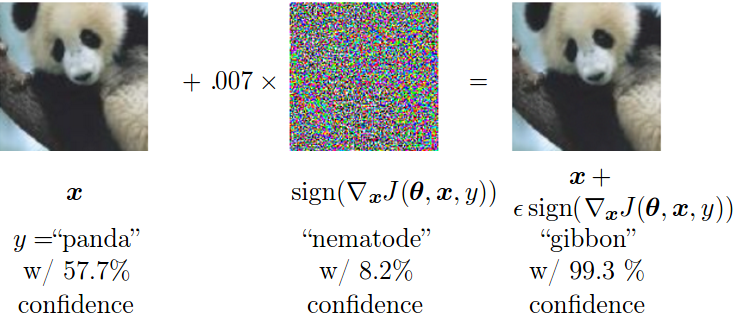
\includegraphics[width=5in]{fig/chap7/7_8.png} 
   \caption{在ImageNet上应用于GoogLeNet(Szegedy等人,2014a)生成对抗样本的演示。通过添加一个不可察觉的小向量,其元素等于损失函数相对于输入的梯度的元素的符号(the sign of the elements),我们可以改变GoogLeNet对图像的分类。经Goodfellow等人许可转载(2014b)。}
   \label{fig:7_8}
\end{figure}

Goodfellow等人(2014b)表明,这些对抗性样本的主要原因之一是过度的线性。神经网络主要由线性构建块构成。在一些实验中,它们实现的总体功能证明是高度线性的。这些线性函数易于优化。不幸的是,如果线性函数具有许多输入,它的值可以非常快速地改变。如果我们通过$\epsilon $改变每个输入,则具有权重$w$的线性函数值可以被越来越大的$\epsilon ||w||_1$改变,如果$w$是高维的,则计算出的值是非常大的。对抗训练通过鼓励网络局部恒定训练数据的邻域(locally constantin the neighborhood of the training data)来阻止这种高度敏感的局部线性行为。这可以被看作是在监督神经网络中显式地引入局部恒定性(local constancy prior)的方式。

对抗训练有助于说明结合使用大型函数家族和积极正则化力量。纯线性模型,如逻辑回归,不能抵抗对抗样本,因为它们是被强制线性的。神经网络能够表示从接近线性到几乎局部常量值的函数,并因此具有捕获训练数据中线性趋势,并同时学习抵抗局部扰动的灵活性。

对抗样本还提供了完成半监督学习的手段。在与数据集中的标签不相关联的点$x$处,模型本身分配一些标签$y$。模型的标签$y$可能不是真实的标签,但是如果模型是高质量的,则$y$具有提供真实标签的高概率。我们可以选找一个对抗样本,使得分类器输出一个$y^{'} \neq y$的标签$y$。使用不是真实标签而是由训练模型提供的标签产生的对抗性样本被称为虚拟对抗性样本(virtual adversarial examples,Miyato等人,2015)。分类器也许会把相同的标签分配给$x$和$x^{'}$。这鼓励分类器学习一个函数,该函数对于未标记数据所在的流形中的任何地方的小变化是鲁棒的。驱动这种方法的假设是不同的类通常位于断开的流形空间上,并且小的扰动不应该能够从一个类的流形空间跳到另一个类的流形空间上。

\section{切线距离与切线传播和流形切线分类器}

许多机器学习算法旨在通过假设数据位于低维流行空间附近来克服维数诅咒,如第5.11.3节所述。

早期利用流形假设的尝试之一是切线距离算法(Simard等人,1993,1998)。它是一种非参数最近邻算法,其中使用的度量不是通用欧几里得距离,而是一种从流形空间衍生出的度量方法,接近概率集中附近的流形空间。假设我们试图对实例进行分类,并且处在同一流形空间的样本具有相同的类别。由于分类器应该对流形空间局部的变化因子保持不变,因此使用点$x_1$和$x_2$之间的最近相邻距离作为它们分别属于的流形$M_1$和$M_2$之间的距离是有意义的。虽然在计算上有困难(需要解决优化问题,找到$M_1$和$M_2$上最接近的点对),但是在局部有意义的一种简便的替代方案是通过其在$x_i$处的切平面近似$M_i$,并且测量两个切线,或者在切平面和点之间策略。这可以通过解决低维线性系统(在流形空间的维度中)来实现。当然,该算法需要指定切向量。

在相关方法中,切线传播算法(Simard等人,1992)(图7.9)训练一个具有额外惩罚的神经网络分类器,使得神经网络的每个输出$f(x)$值局部地对变化因子保持不变性。这些变化因子对应于沿着流形的移动,相同类别的样本在该流形空间的附近集中。局部不变性通过要求$\triangledown_x f(x)$与$x$处的已知流形空间的切向量$v^{(i)}$正交来实现,或者等效地,在方向$v^{(i)}$位于样本$x$处的$f$的方向导数,通过增加正则化惩罚$\Omega$:
$$
\begin{aligned} \label{eq:767}
\Omega(f) = \sum_i \Big((\nabla_{x} f(x)^\top v^{(i)}) \Big)^2 .
\end{aligned}
$$
这个正则化器当然可以通过适当的超参数缩放,并且对于大多数神经网络,我们将需要对许多输出求和,而不是这里为了简单起见描述的单个输出$f(x)$。与切线距离算法一样,切向量通常是从图像中的变换效果(例如平移,旋转和缩放)的形式知识这样的先验推导出来的。切线传播不仅用于监督学习(Simard等人,1992),而且也适用在强化学习的背景下(Thrun,1995)。

切线传播与数据集扩增(data augmentation)密切相关。在这两种情况下,在不改变网络原本样本的输出情况下,算法使用者将指定一系列数据集图像扩增来获取更多图像数据,并在此过程中考虑该任务的先验知识。不同的是,在数据集增加的情况下,网络被显式地训练以正确地分类通过对原始图像变换从而创建的极少的不同输入。切线传播不需要显式访问新的输入点。相反,它分析地正则化模型以抵抗在与变换相对应方向上的扰动。虽然这种分析方法在理智上是优雅的,但它有两个主要的缺点。首先,它只是将模型正则化以抵抗极少的扰动。显式数据集赋予模型对较大扰动的抵抗力。第二,极少数方法对基于校正线性单元(ReLU)的模型造成了不利影响。这些模型只能通过关闭单元或缩小其权重来收缩其导数。它们不能通过以大的权重以高的值饱和而收缩它们的导数值,如S型或$tanh$激活函数。数据集增加可与线性校正单元(ReLU)很好地兼容,因为线性校正单元(ReLU)的不同子集可以激活每个原始输入的不同变换版本。

\begin{figure}[htbp] %  figure placement: here, top, bottom, or page
   \centering
   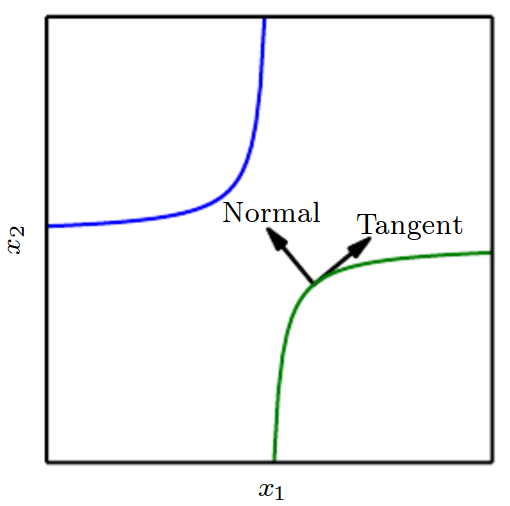
\includegraphics[width=3in]{fig/chap7/7_9.png} 
   \caption{该图描述了正切传播算法(Simard等人,1992)和流形正切分类器(Rifai等人,2011c)的主要思想,它们都对分类器的输出函数$f(x)$正则化。每条曲线表示不同类别的流形空间,这里显示的是嵌入在二维空间中的一维流形空间。在一个曲线中,我们选择单个点并绘制与该类相切的向量(平行于并且接触流形空间)和垂直于类流形空间(与流形空间正交)的向量。在多个维度中,可以存在许多切线方向和许多法线方向。我们期望分类函数随着其在垂直于流形的方向上移动而快速改变,并且不随着其沿类流形空间移动而改变。切向传播和流形切线分类器正则化$f(x)$不随着$x$沿流形移动而改变很多。流形切线分类器通过训练自动编码器来拟合训练数据来估计流形切线方向,切向传播需要用户手动指定计算切线方向的函数(例如在相同类的流形中指定图像的小平移保持)。使用自动编码器估计流形将在第14章中描述。}
   \label{fig:7_9}
\end{figure}

切线传播也与\textbf{双重反向传播}(Drucker和LeCun,1992)、对抗训练(Szegedy等人,2014b;Goodfellow等人,2014b)有关。双重反向传播的正则会使Jacobian矩阵变小,而对抗训练在原始输入附近找与之接近的输,并训练模型产生与原始输入一样的输出。切线传播和指定变化方法的数据集扩增这两个策略都要求模型对于输入中的某些指定的变化方向具有一定的不变性。只要变化很小,双重反向传播和对抗训练在模型对输入样本在所有变化方向都有不变性。正如数据集扩增是切线传播的非极少数版本,对抗训练是双重反向传播的非极少数版本(Just as dataset augmentation is the non-infinitesimal version of tangent propagation, adversarial training is the non-infinitesimal version of double backprop.)。

流形切线分类器(Rifai等人,2011c),消除了需要知道切向量的这一先验。如我们将在第14章中看到的,自动编码器可以估计流形切线向量。流形切线分类器使用这种技术,以避免需要用户指定切向量。如图14.10所示,这些估计的切线向量超出了由图像的几何形状(例如平移,旋转和缩放)产生的经典不变量,并且包括因为是特定对象的(例如移动身体部分),也是必须被学习的因素。因此,用流形切线分类提出的算法很简单:(1)使用自动编码器通过无监督学习来学习流形结构,(2)使用这些切线在切线传播中正则化神经网络分类器(方程7.67)。

本章描述了用于正则化神经网络的大多数策略。正则化是机器学习的中心主题,因此其余正则化策略将定期重新讨论。机器学习的另一个中心主题是优化,见下一章节。